% This report was inspired from templates-
% 1. https://www.overleaf.com/latex/templates/thesis-template-faculty-of-computer-science-university-of-vienna/whyzmtqggxzz
% 2. https://www.overleaf.com/latex/templates/synopsis-template-university-of-hyderabad/fknzkwvjbhfx
\DeclareOldFontCommand{\bf}{\bfseries}{\textbf}
\let\cleardoublepage\clearpage

\documentclass[oneside, hidelinks]{UniVieCS_Thesis}
\input{packages_macros}
\makeglossaries
\KOMAoptions{open=any}
\usepackage[ngerman, british]{babel}
\usepackage{amssymb}
\renewcommand*\chapterheadstartvskip{\vspace*{0pt}}

\usepackage{tikz}
\newcommand{\circledU}{%
  \tikz[baseline=(char.base)]{
    \node[shape=circle,draw,inner sep=0.5pt] (char) {$\scriptscriptstyle U$};
  }%
}
\usepackage{float}
\usepackage{caption}
\captionsetup[figure]{skip=5pt}
\usepackage{enumitem}
\usepackage{wrapfig}
\usepackage{fancyhdr}
\pagestyle{fancy}
\fancyhf{}

\fancyhead[L]{\nouppercase{\leftmark}}
\fancyhead[R]{\thepage}              
\renewcommand{\headrulewidth}{0.4pt}   
\renewcommand{\footrulewidth}{0pt}    

\fancypagestyle{plain}{
    \renewcommand{\footrulewidth}{0pt}
}

\begin{document}

    \thispagestyle{empty}
\begin{center}
    {\Huge\bf{Gomory-Hu Tree} \\}

    \vspace{3cm}
    {\large \bf Soham Chakraborty \\
    22CS02002\\}

    \vspace{2cm}
    {\Large{\bf B.Tech and M.Tech (Dual Degree) \\ in \\Computer Science and Engineering\\ Semester 8\\}}

    \vspace{2cm}
    {\bf\textit{Under the supervision of\\ }}
    {\Large{\bf Dr. Joy Chandra Mukherjee}\\}

    \vspace{1cm}
    
\includegraphics[width=0.30\linewidth]{figures/logo_iit_bbs.png}

    \vspace{1cm}
    {\large\bf School of Electrical and Computer Sciences\\}
    {\large\bf Indian Institute of Technology Bhubaneswar \\}
    {\large\bf May 2026 }
\end{center}

    
    \clearpage
	\frontmatter{}
	\begin{titlepage}
    % --------- Abstract ---------
    
    \begin{center}
    {\LARGE \bfseries Abstract}
    \end{center}
    \vspace{-7mm}
    {\centering
        \rule{0.9\textwidth}{1pt}
    \par}
    \vspace{7mm}
    
    \begin{center}
    \begin{minipage}{0.9\textwidth}

    \large{
    Computing the maximum network flow for all pairs of nodes in an undirected graph and can be trivially done using a brute force approach with $\binom{n}{2}$ flow computations. First, we discuss about an algorithm proposed by Gomory-Hu [GH61] which solves this problem using only $n-1$ flow computations. Then, we discuss about construction and use of Dynamic Gomory-Hu trees as proposed by T. Hartmann and D. Wagner [HT13], which handles single edge weight updates, insertion and deletion in an efficient manner. \\
    We then explore a specific application of Gomory-Hu Tree: Image Segmentation and a Hierarchical Cut-based Clustering algorithm used for Image Segmentation proposed by Zhenyu Wu and Richard Leahy [WL93]. I then provide/present some improvements over the proposed algorithm for better Clustering and Execution Time improvements. \\
    Finally, we conclude with the Advantages and Drawbacks of the above algorithm and Future Work possibilities in the domain of Gomory-Hu Tree.
    }
    \end{minipage}
    \end{center}

    % --------- Acknowledgements ---------

    \vspace*{3cm}
    \begin{center}
    {\LARGE \bfseries Acknowledgements}
    \end{center}
    \vspace{-7mm}
    {\centering
        \rule{0.9\textwidth}{1pt}
    \par}
    \vspace{7mm}
    
    \begin{center}
    \begin{minipage}{0.9\textwidth}

    \large{
    I have a very keen interest in the field of Data Structures and Algorithms. I am grateful to Joy Sir for giving me a BTP topic related to my interest in Algorithms and weekly interaction about insights into further developments and follow-ups of the project. Competitive programming being my favourite domain and C++ as the primary programming language it was a nice experience converting Pseudo-codes from various research papers in functioning C++ codes (with not so nice experience of debugging). Being a Dual Degree student, I have 3 more semesters before I graduate and in this time I wish to further develop this project and make some progress into other related topics with the help of Joy Sir to a full-fledged MTP project.
    }
    
    \end{minipage}
    \end{center}

    \vfill
\end{titlepage}
	\pagebreak
	
    \microtypesetup{protrusion=false}
    \tableofcontents{} 
    
    \textbf{\newline C++ implementation --}
    \href{https://github.com/soham-c04/Gomory-Hu-Tree}{\textcolor{blue}{Github Repo}}
    
    \cleardoublepage{}
    \microtypesetup{protrusion=true}
    
	\pagebreak
	
	\mainmatter{}
    \chapter{Introduction}
    In this project, we look at algorithms for solving graph-theoretic problems related to Multi-Terminal minimum cut - maximum flow in a network. It consists of 4 parts - 
    \begin{enumerate}
        \item {Gomory-Hu Cut Tree}
        \item {Modified Cut-Tree algorithm by Gusfield}
        \item {Dynamic Gomory-Hu Tree}
        \item {Future Work}
    \end{enumerate}

    \section{Overview}
    We here give a brief insight to the first 3 parts from above.
    
    \vspace{5mm}
    \noindent{\large\bf Part I: Gomory-Hu Tree\\[1mm]}
    A Gomory-Hu tree is an undirected, weighted tree on the vertices of a given graph such that each edge in the tree represents a minimum separating cut in the underlying graph with respect to its incident
    vertices. The cost of the cut is given by the cost of the tree edge. From this property it follows directly that a minimum separating cut for two vertices that are not adjacent in the tree is given by a cheapeast tree edge on the unique path between both vertices. We first give a description of the very first algorithm proposed by Gomory and Hu for constructing a Cut-Tree on general graphs and explain the ideas and mechanisms it relies on. This lays the basics for newer algorithmic approaches to constructing Cut-Trees such as the one given by Gusfield in Part II.

    \vspace{5mm}
    \noindent{\large \bf Part II: Implementation of Cut Tree by Gusfield\\[1mm]}
    Gusfield provides an algorithm that constructs the Gomory-Hu Tree in an extremely easy manner by extrapolating some relaxations in the inital construction for the maintainence of Gomory-Hu Tree formation. We start with describing the Equivalent Flow Tree Program, after which adding just a single \textit{if statement} gives us a Cut Tree. Further, he shows that adding one more line of \textit{for loop} into the code computes the complete All-Pair Max. Flow matrix.

    \vspace{5mm}
    \noindent{\large \bf Part III: Dynamic Gomory-Hu Tree\\[1mm]}
    The Dynamic Gomory-Hu Tree as proposed by Tanja Hartmann and Dorothea Wagner aims at maintaining Gomory-Hu trees also in evolving graphs. We consider a dynamic scenario where two cases of the underlying graph differ due an atomic edge change\footnote[1]{Edge weight increase, Edge weight decrease, edge insertion and edge deletion}. In the incremental scenarios, we are interested in updating the Gomory-Hu tree each time as efficiently as possible, as compared to constructing the whole tree from scratch.  
    \enlargethispage{\baselineskip}

     \section{Notations and Definitions on Graphs}
     In this section, we present the notation used throughout the report and give definitions of most terms that occur. Some of the incidentally mentioned concepts however, are mentioned on that point only.

    \vspace{5mm}
    \noindent{\large \bf Undirected Graphs:} Apart from maximum flows which are usually considered in \textit{directed} graphs we only consider weighted \textit{undirected} graphs here. An undirected,weighted graph is a graph $G = (V,E,c)$ with vertices $V$, edges $E$ and a positive edge cost function $c:E\xrightarrow{}{R_0}^{+}$, writing $c(u,v)$ as a shorthand for $c({u,v})$ with $\{u,v\} \in E$. We will also be using $n:=|V|$ and $m:=|E|$ as obvious notations which will be clear from the context.

    \vspace{5mm}
    \noindent{\large \bf Special Cases:} We define a \textit{simple path} of $n$ vertices as a sequence $v_1,v_2,...,v_n$ of vertices such that $v_i \ne v_j$ for $i \ne j$, $\{i,j\}\subseteq {1,2,...,n}$ and $\{v_i,v_j\}$ forms an edge for $i=1,2,...,n-1$. A \textit{tree} is a connected acyclic graph. The path between two vertices of a tree is unique, and we write $\pi (u,v)$ for the path between $u$ and $v$.

    \vspace{5mm}
    \noindent{\large \bf Dynamic Graphs:} We call a graph \textit{dynamic} if its edges vary over time. Assume, change in graph $G$ either involves an edge $\{b,d\}$ with $c(b,d)= \Delta > 0$. If the cost of $\{b,d\}$ in $G$ decreases by $c(b,d) = \Delta > 0$, edge is deleted and resulting graph is termed $G^{\mathbin{\large\ominus}}$. Similarly, inserting $\{b,d\}$ or increasing the cost yields $G^\oplus$. We denote the cost function after a change by $c^{\mathbin{\large\ominus}}$ and $c^\oplus$ respectively. If we consider the graph after an arbitrary change, without any further information about the type of change, we denote it by $G^{\circledU}$ 
    
    \section{Cuts and Flows}
    A \textit{cut} in an undirected weighted graph $G = (V,E,c)$ is a partition of $V$ into two non-empty \textit{cut sides} $S$ and $V \backslash S$. The cost $c(S,V \backslash S)$ of a cut in $G$ is the sum of the costs of all edges \textit{crossing} the cut, that is, edges $\{u,v\}$ with $u \in S, v \in V\backslash S$ also denoted as $c(S)$. A \textit{cut set} is the set of edges crossing the cut. Two cuts are said to be \textit{nested} if their cut sides are nested and \textit{non-crossing} if their cut sides are nested or the two cut sides are disjoint. A set of cuts is called \textit{non-crossing} if all cuts are pairwise non-crossing. A \textit{minimum u-v-cut} is a cut that separates \textit{u} and \textit{v} and is the cheapest cut among all cuts separating these vertices, denoted by $\lambda (u,v)$.

    
    From equivalence of $\lambda (u,v)$ and the \textit{value of maximum u-v-flow} in an undirected, weighted graph as stated by Ford-Fulkerson, computing minimum \textit{u-v}-cut in an undirected, weighted graph is basically same as computing maximum \textit{u-v-}flow in this graph. The best known complexity for solving the \textit{max flow - min cut} problem is $O(nm + n^2\log n$ by Nagamochi and Ibaraki.

    \textbf{Flow} in $G$ between two vertices $s$ and $t$ is a function $f:E\xrightarrow{}R_0^{+}$ that satisfies:
    \begin{enumerate}
        \item {$f(e) \le c(e), \forall e\in E$}
        \item {$\sum_{x\in N_i(v)}f(x,v) = \sum_{y\in N_o(v)}f(v,y), \forall v \in V\backslash \{s,t\}$}
    \end{enumerate}
    \chapter{Gomory-Hu Tree}
    \section{Definition}

    {\large \bf Gomory-Hu Tree} is a weighted tree $T(G) = (V,E_T,c_T)$ on the vertices of an undirected (weighted) graph $G = (V,E,c)$ (with edges not necessarily in $G$) such that each $\{u,v\}\in E_T$ induces a minimum \textit{u-v-}cut in $G$ *by decomposing $T(G)$ into two connected components) and such that $c_T(\{u,v\})$ is equal to the cost of the induced cut. The cuts induced by $T(G)$ are non-crossing and for each $\{s,t\} \subseteq V$ each cheapest edge on the path $\pi (u,v)$ between $s$ and $t$ in $T(G)$ corresponds to a minimum \textit{s-t-}cut in $G$. A Gomory-Hu tree thus represents $n-1$ non-crossing minimum \textit{s-t-cuts}.
    
    \textit{Reconnecting} an edge in $T(G)$ means replacing the edge by another edge with the same attributes without creating a cycle. \textit{Step pairs} refers to the cut pairs that are considered for the computation of minimum separating cuts during the construction.

    \vspace{5mm}
    {\large \bf Flow-Equivalent Tree} is a weighted tree $T(G) = (V,E_T,c_T)$ on the vertices of $G$ having cost function $c_T:E_T\xrightarrow{}R_0^{+}$ such that the cost $c_T(\{s,t\})$ of each edge $\{s,t\}$ corresponds to $\lambda_G (s,t)$. Hence, it also holds that edge connectivity $\lambda_G (s,t)$ for an arbitrary vertex pair $\{s,t\}\subseteq V$ is given by the cost of the cheapest edge on teh path between $s$ and $t$ in $T(G)$ i.e. $\lambda_{T(G)} (s,t) = \lambda_G (s,t)$. Hence, Gomory-Hu trees are a subclass of flow-equivalent trees.

    \section{Construction algorithm}

    {\large \bf Lemma 2.1:} \textit{A set $\mathcal{H}$ of $n-1$ cuts is a Gomory-Hu set if and only if the cuts in $\mathcal{H}$ are pairwise non-crossing and for each cut exists a cut-pair that is exclusively separated by this cut, that is, not separated by any other cut in $\mathcal{H}$.}
    
    \vspace{3mm}
    \noindent\textit{Proof:} Clearly, each Gomory-Hu tree satisfies the conditions of Lemma 2.1. Now let $\mathcal{H}$ denote a set of $n-1$ pairwise non-crossing cuts and $\mathcal{P}$ a set of $|\mathcal{H}|$ exclusively separated cur pairs. Since cuts in $\mathcal{H}$ are non-crossing, their cuts are nested, and since there are $n-1$ of these cuts, there exists exactly one vertex pair for each cut that is exclusively separated by this cut. Hence, these vertex pairs must correspond to the cut pairs in $\mathcal{P}$. Connecting cut pairs in $\mathcal{P}$ by edges then yields a Gomory-Hu tree that represents $\mathcal{H}.$

    \vspace{5mm}
    \noindent{\large \bf Lemma 2.2:} (Non-Crossing Lemma) \textit{Let $(X,V\backslash X)$ be a minimum x-y-cut in G, with $x\in X$. Let $(H,V\backslash H)$ be a minimum u-v-cut, with $u,v\in V\backslash X$ and $x\in H$. Then the cut $(H\cup X, (V\backslash H)\cap (V\backslash X))$ is also a minimum u-v-cut.}
    \vspace{5mm}

    \noindent The idea of the Algorithm proposed by Gomory and Hu is to iteratively construct a Gomory-Hu set by choosing in each step a vertex pair (\textit{step pair}) that is not yet separated and computing a minimum separating cut for this pair. To ensure that each cut is non-crossing (from Lemma 2.1) Gomory and Hu contract at least one cut side of each cut found so far and compute the minimum separating cut in the resulting graph. This is due to the result of Lemma 2.2 (Non-Crossing Lemma) that there always exists a minimum separating cut that does not cross any of the previous cuts. 
    
    The following pseudocode is for the Algorithm 1 by Gomory and Hu for the construction of Cut-Tree. The \textit{intermediate tree} $T_* = (V_*,E_*,c_*)$ is initialized as an isolated, edgeless node containing all original vertices. Then, until each node of $T_*$ is a singleton node, a node $S\in V_*$ is \textit{split} and an edge representing a new cut ia added to $E_*$. Now, supernodes $S'\ne S$ which are related to cut sides of previously found cuts, are dealt with by contracting in G whole subtrees $N_j$ of $S$ in $T_*$, connected to $S$ via edges $\{S,S_j\}$, to single nodes $[N_j]$ before cutting, whihc yields $G_S$. The split of $S$ into $S_u$ and $S_v$ is then defined by a minimum u-v-cut (split cut) in $G_S$ (with \textit{step pair} $\{u,v\} \subseteq S$), which does not cross any of the previously used cuts due to the contraction technique. Reacll that this split cut in $G_S$ also induces a minimum \textit{u-v-}cut in $G$, due to the Non-Crossing Lemma (2). After splitting, the edge $\{S_u,S_v\}$ is added to $E_*$, and each $N_j$ is reconnected, again by $S_j$, to either $S_u$ or $S_v$ depending on which side of the cut $[N_j]$ ended up. This reconnection ensures that the edge $\{S_u,S_v\}$ indeed represents the split cut.

    \vspace{5mm}
    \begin{algorithm}[H]
        \hrulefill
        
        \textbf{Algorithm 1:} Gomory--Hu
        
        \hrulefill
        \vspace{2mm}
        
        \DontPrintSemicolon
        
        \KwIn{Graph $G = (V,E,c)$}
        \KwOut{Gomory--Hu tree of $G$}
        
        Initialize $T_* := (V_*, E_*, c_*)$ with $V_* \gets \{V\}$, $E_* \gets \varnothing$, $c_*$ empty\;
        
        \While{$\exists S \in V_* \text{ with } |S| > 1$}{
            $\{u,v\} \gets$ arbitrary pair in $S$ \tcp*{unfold node}
        
            \ForEach{$S_j$ adjacent to $S$ in $T_*$}{
                $N_j \gets$ subtree of $S$ in $T_*$ with $S_j \in N_j$\;
            }
        
            $G_S = (V_S,E_S,c_S) \gets$ contract each $N_j$ to $[N_j]$ in $G$ \tcp*{contraction}
        
            $(U, V \setminus U) \gets$ min-$u$-$v$-cut in $G_S$, cost $\lambda_{G_S}(u,v)$\;
        
            $S_u \gets S \cap U$, \quad $S_v \gets S \cap (V_S \setminus U)$ \tcp*{split $S = S_u \cup S_v$}
        
            $V_* \gets (V_* \setminus \{S\}) \cup \{S_u, S_v\}$\;
        
            $E_* \gets E_* \cup \{\{S_u,S_v\}\}$\;
            $c_*(S_u,S_v) \gets \lambda_{G_S}(u,v)$\;
        
            \ForEach{former edges $e_j = \{S, S_j\}$ in $E_*$}{
                \eIf{$[N_j] \in U$}{
                    $e_j \gets \{S_u, S_j\}$ \tcp*{reconnect to $S_u$}
                }{
                    $e_j \gets \{S_v, S_j\}$ \tcp*{reconnect to $S_v$}
                }
            }
        }
        
        \Return{$T_*$}\;
        
        \vspace{2mm}
        \hrulefill
    \end{algorithm}

    \enlargethispage{\baselineskip}
    \enlargethispage{\baselineskip}

    \chapter{Modified Cut-Tree algorithm by Gusfield}
    Gomory and Hu in their implementation of Cut-Tree use contractions in G to prevent crossings of the cuts. Gusfield provides a simplified version of the same by relaxing the above conditions and arbitrarily separating cuts directly in G without any contractions. Gusfield in his implementation resolves non-crossing cuts using the Non-Crossing Lemma (2). To maintain the reconnection of edges in the \textit{Intermediate Tree} he uses a parent array and another array to represent the weight from a vertex to its parent.

    \section{Intermediate Trees}
    An intermediate tree is a partially formed Gomory-Hu Tree which has not yet completed all the $n-1$ iterations to reach the final state. In an Intermediate Tree represented by $T_* = (V_*,E_*,c_*)$ each node in $V_*$, which consists of original vertices in $V$, by an arbitrary tree of \textit{thin} edges connecting the contained vertices in order to indicate their membership to the node. An edge connecting two nodes in $V_*$ is represented by a \textit{fat} edge in $E_*$, which we connect to an arbitrary vertex in each incident node. Fat edges represent minimum separating cuts in G, and are thus associated with costs. If a node contains only one vertex, we color this vertex black. Black vertices are only incident to at least one thin edge. In this way, $T_* = (V,E_t,E_f,c_f)$ can be also considered as a tree on $V$ with two types of edges (thin edges in $E_t$, fat edges in $E_f$) and vertices (black and white), and a cost function $c_f$ on the fat edges. See figure below:
    
    \begin{figure}[!htb]
        \centering
        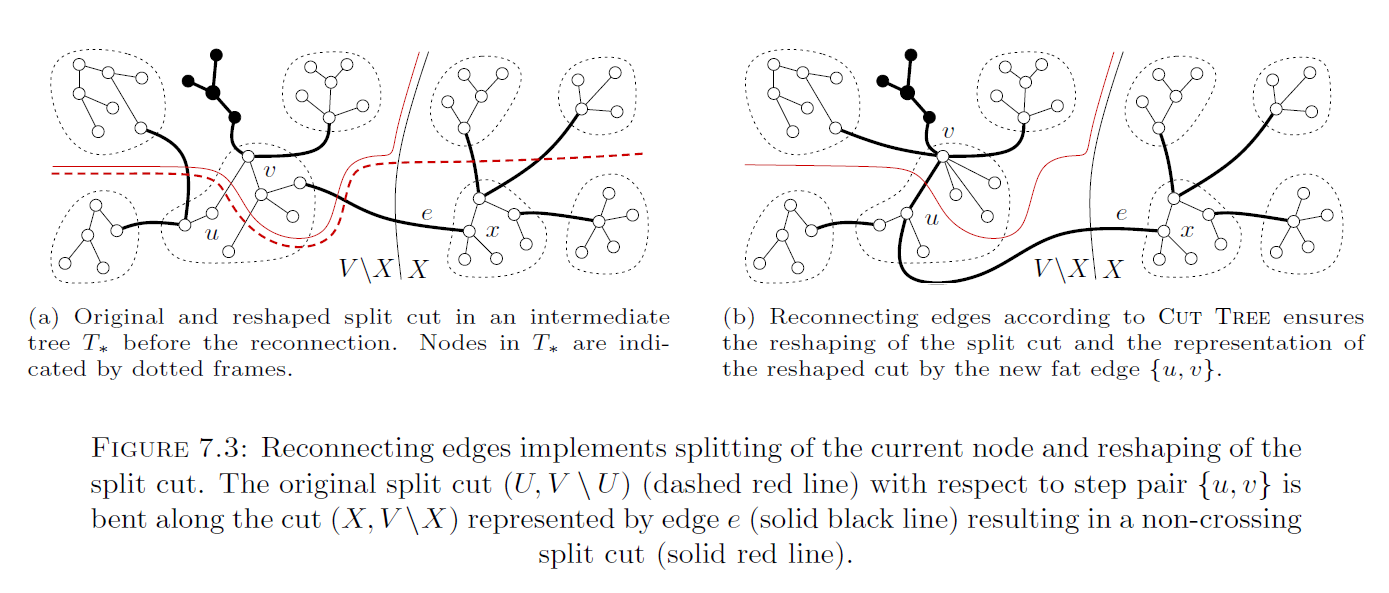
\includegraphics[width=\linewidth]{figures/thin_fat.png}
    \end{figure}

    \section{Description}
    From the above addressing of subtrees of a node using arrays in $T_*$ we can easily address the vertices that are linked by a fat edge to a vertex in the node. As per the representation described above, Algorithm 2 considers the intermediate tree $T_*$ as a tree on the vertices of $G$ consisting of thin and fat edges and bypasses any contraction in $G$. Now, modify Algorithm 1 so that in every intermediate tree, every supernode S contains exactly one node called the \textit{parent/representative} of S, denoted $r(S)$. Then any one node is arbitrarily chosen to be the representative of the first supernode of GH method (Algorithm 1). Next, each successive flow is computed between $r(S)$ and some other vertex $v\in S$. S is split into two supernodes $S_{r(S)}$ and $S_v$. Assign $r(S)$ as the representative of $S_{r(S)}$, and $v$ to be the representative of $S_v$. If $S'$ is a supernode neighbor of $S$ in $T$ before the split, and $r(S')$ falls on the $v$ side of the cut, then replace the $(S,S')$ edge with edge $(S_v,S')$. Now, after $n-1$ iterations each supernode decomposes into a node having only 1 vertex each.

    \vspace{2cm}
    \begin{algorithm}[H]
        \hrulefill
        
        \textbf{Algorithm 2:} Modified Cut-Tree
        
        \hrulefill
        \vspace{2mm}

    \DontPrintSemicolon
    
    \KwIn{Graph $G = (V,E,c)$}
    \KwOut{Cut tree of $G$}
    
    \For{$s \gets 2$ \KwTo $n$}{
        
        Compute a minimum cut between nodes $s$ and $t := p[s]$ in $G$.\;
        Let $X$ be the set of nodes on the $s$-side of the cut.\;
        Output the maximum $s,t$ flow value $f(s,t)$.\;
        
        $fl[s] \gets f(s,t)$\;
    
        \For{$i \gets 1$ \KwTo $n$}{
            \If{$(i \neq s)$ \text{ and } $i \in X$ \text{ and } $p[i] = t$}{
                $p[i] \gets s$\;
            }
        }
    
        \If{$p[t] \in X$}{
            $p[s] \gets p[t]$\;
            $p[t] \gets s$\;
    
            $fl[s] \gets fl[t]$\;
            $fl[t] \gets f(s,t)$\;
        }
    }
    \vspace{2mm}
    \hrulefill
    
    \end{algorithm}


    
    
    \chapter{Dynamic Gomory-Hu Tree}
    Here we seek methods to efficiently maintain a Gomory-Hu Tree also in a dynamic scenario, where the underlying graph changes over time. We consider changes in the GH tree that occurs when a concrete change occurs on a concrete edge. Similar work has been done in context of \textit{sensitivity analysis of multi-terminal flow networks} by Elmaghraby and \textit{parametric maximum flows.} by Gallo et al. and Scutella.

    \section{Finding Reusable Cuts}
    
    The main idea of this approach is to determine cuts in a given Gomory-Hu tree $T(G)$ that are still minimum separating cuts in the graph $G^{\circledU}$ after a change, and thus, can be reused for the construction of a new Gomory-Hu tree $T(G^{\circledU})$. If an old cut is not reusable with respect to this some checked vertex, then using this method it is not guaranteed that the cut won't also be reusable with respect to some other vertex. Below are some \textbf{Lemmas} and \textbf{Corollaries} to detect reusable cuts.

    \vspace{5mm}
    \noindent{\large \bf Lemma 4.1:} \textit{If $c(b,d)$ changes by $\Delta >0$, then each $\{u,v\}\in E_T$ remains a minimum u-v-cut (i) in $G^\oplus$ with cost $\lambda_G(u,v)$ if $\{u,v\}\notin \pi(b,d)$, (ii) in $G^\ominus$ with cost $\lambda_G(u,v)-\Delta$ if $\{u,v\}\in \pi(b,d)$.}

    \begin{figure}[!htb]
        \centering
        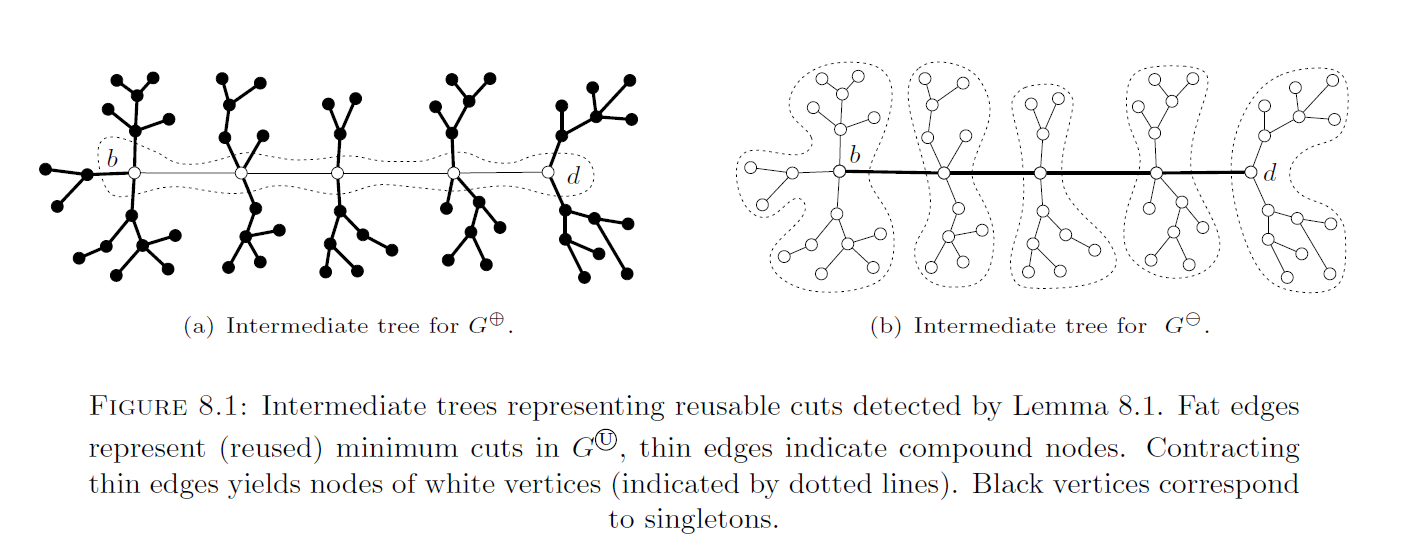
\includegraphics[width=\linewidth]{figures/G+G-.png}
        \label{GplusGminus}
    \end{figure}

    \vspace{5mm}
    \noindent{\large \bf Corollary 4.1:} \textit{If $\{b,d\}$ is newly inserted with $c^\oplus (b,d) = \Delta$ or $c(b,d)$ increases by $\Delta$, any minimum b-d-cut in $G$ remains valid in $G^\oplus$ with $\lambda_{G^\oplus}(b,d) = \lambda_G(b,d)+\Delta$.}
    \vspace{3mm}
    
    \noindent Corollary 4.1 directly allows us to use the whole Gomory-Hu tree $T(G)$ if $\{b,d\}$ is an existing bridge in $G$ with increasing cost.

    \vspace{4mm}
    \noindent{\large \bf Corollary 4.2:} \textit{An edge $\{u,v\}$ is a bridge in $G$ if and only if $c(u,v) = \lambda_G(u,v) >0$. Then $\{u,v\}$ is also an edge in $T(G)$.}

    \vspace{5mm}
    \noindent{\large \bf Lemma 4.2:} \textit{Let $\{b,d\}$ be a new bridge in $G^\oplus$. Then replacing an edge of cost 0 on $\pi (b,d)$ in $T(G)$ by $\{b,d\}$ with cost $c^\oplus (b,d)$ yields a new Gomory-Hu tree $T(G^\oplus)$.}

    \vspace{5mm}
    \noindent{\large \bf Lemma 4.3:} \textit{If $\{b,d\}$ is a bridge in $G$ and the cost decreases by $\Delta$ (or $\{b,d\}$ is deleted), decreasing all edge costs on $\pi (b,d)$ in $T(G)$ by $\Delta$ yields a new cut tree $T(G^\ominus)$.}
    \vspace{3mm}

    \noindent Lemma 4.3 allows us to easily handle edge weight decrease in bridges with 0 new flow computations.
    
    \vspace{5mm}
    \noindent{\large \bf Corollary 4.3:} \textit{Let $\{u,v\}$ denote an edge in $T(G)$ with $c_T(u,v)=0$ or an edge that corresponds to a bridge in $G$. Then $\{u,v\}$ is still a minimum u-v-cut in $G^\ominus$.}

    \vspace{5mm}
    \noindent{\large \bf Lemma 4.4:} \textit{Let $(U,V\backslash U)$ be a minimum u-v-cut in $G^\ominus$ with $\{b,d\}\subseteq V\backslash U$ and let $\{g,h\}\in E_T$ be an edge in $T(G)$ with $g,h\in U$. Then $\{g,h\}$ is a minimum separating cut in $G^\ominus$ for all its previous cut pairs within $U$.}
    \vspace{3mm}

    \noindent Lemma 4.4 allows us to reuse all edges in $E_T$ that lie on a common side of the cut.
    
    \vspace{5mm}
    \noindent{\large \bf Lemma 4.5:} \textit{Let $T_* = (V,E_*,c_*)$ denote a valid intermediate tree for $G^\ominus$, where all edges on $\pi (b,d)$ are fat and let $\{u,v\}$ be a thin edge with $v$ on $\pi (b,d)$ such that $\{u,v\}$ represents an old minimum u-v-cut in G. Let $N_\pi$ denote the set of neighbors of $v$ on $\pi (b,d)$. If $\lambda_G (u,v) \le min_{x\in N_\pi}\{c_*(x,v)\}$}, then $\{u,v\}$ is a minimum u-v-cut in $G^\ominus$.

    \section{Algorithm}
    Here we will show two update algorithms one for increase in edge costs or edge insertions and another for decrease in edge costs or edge deletion. Below in both cases it is assumed that the edge being updated is $\{b,d\}\in E$ with $\Delta >0$.

    \subsection{Increasing Edge Costs}
    If $\{b,d\}$ is an existing bridge or newly inserted bridge in $G$, then it adapts $c_T (b,d)$ according to Corollary 4.1.
    Otherwise, if $\{b,d\}$ is a newly inserted bridge in $G$, it rebuilds $T(G)$ according to Lemma 4.2. In both cases they require no new cut-computations.

    If $\{b,d\}$ is not a bridge we create the intermediate tree as in Figure~\ref{GplusGminus}(a) reusing all edges not in $\pi (b,d)$. Then as per Figure~\ref{GplusGminus}(a) we create an intermediate tree by compressing all vertices on the path $\pi (b,d)$ into a supernode and decomposing the supernode using a slightly modified version of Algorithm 2.

    \begin{algorithm}[H]
    \hrulefill
    
    \textbf{Algorithm 3:} Increase or Insert
    
    \hrulefill
    \vspace{2mm}
    
    \DontPrintSemicolon
    
    \KwIn{$T(G),\, b,d,\, c(b,d),\, c^{\oplus}(b,d),\, \Delta :=  c^{\oplus}(b,d)-c(b,d)$}
    \KwOut{$T(G^{\oplus})$}
    
    $T_{\star} \gets T(G)$\;
    
    \If{$\{b,d\}$ is a new bridge}{
        Remove an edge on $\pi (b,d)$ with cost = 0\tcp*{Lemma 4.2}
        Add edge $\{b,d\}$ with cost =$c^\oplus (b,d)$
        
        \Return{$T(G^{\oplus}) \gets T_{\star}$}
    }
    \ElseIf{$\{b,d\}$ is an existing bridge}{
        $c_*(b,d)\xleftarrow{}\lambda(b,d) +\Delta$\tcp*{Corollary 4.1}
        \Return{$T(G^{\oplus}) \gets T_{\star}$}
    }
    Construct an intermediate tree according to Figure~\ref{GplusGminus}(a)\;
    
    \Return{$T(G^{\oplus}) \gets CutTree(T_{\star})$}\;\tcp*{Algorithm 1 could also have been used}
    
    \vspace{2mm}
    \hrulefill
    \end{algorithm}

    \vspace{1cm}
    
    \subsection{Decreasing Edge Costs}
    Algorithm 4 for Decrease or Deletion of edges starts by checking if $\{b,d\}$ is a bridge, and if so then reuses the whole Gomory-He tree $T(G)$ with adapted cost $c_T(b,d)$ (Lemma 4.3). Otherwise, it constructs the intermediate tree $T_*$ as shown in Figure~\ref{GplusGminus}(b), reusing all edge on $\pi (b,d)$ with adapted costs. Then it proceeds with iterative steps where the cut pairs are chosen starting with those which have an incident vertex on $\pi (b,d)$. In this way each edge $\{u,v\}$ is found to remain valid to retain the maximal subtree (Lemma 4.4).

    \vspace{5mm}
    \noindent{\large \bf Lemma 4.6:} \textit{Let $(X,V\backslash X)$ denote a minimum x-y-cut in $G$ with $x\in X, y\in V\backslash X$ and $\{b,d\}\subseteq V\backslash X$. Let $(U,V\backslash U)$ denote a further cut. If (i) $(U,V\backslash U)$ separates $x,y$ with $x\in U$, then $c^\ominus(U\cup X,V\backslash (U\cup X))$. If (ii) $(U,V\backslash U)$ does not separate $x,y$ with $x\in V\backslash U$, then $c^\ominus(U\backslash X,V\backslash(U\backslash X)) \le c^\ominus(U,V\backslash U)$.}
    \vspace{5mm}
    
    \noindent We assume that $G$ and $G^\ominus$ are global variables. $\pi (b,d)$ is assumed to be implicitly updated at each step of the iteration. Thin edges are weighted by the old connectivity, fat edges by the new connectivity of their incident vertices. Whenever an edge is reconnected (by reconnecting one of its incident vertices), the newly occurring edge inherits the cost and the thickness from the disappearing edge. Below is the implementation of Algorithm 4:
    
    \clearpage
    \begin{algorithm}[H]
    \vspace{1cm}
    \hrulefill
    
    \textbf{Algorithm 4:} Decrease or Delete
    
    \hrulefill
    \vspace{2mm}
    
    \DontPrintSemicolon
    
    \KwIn{$T(G),\, b,d,\, c(b,d),\, c^{\ominus}(b,d),\, \Delta := c(b,d) - c^{\ominus}(b,d)$}
    \KwOut{$T(G^{\ominus})$}
    
    $T_{\star} \gets T(G)$\;
    
    \If{$\{b,d\}$ is a bridge}{
        \Return{$T(G^{\ominus}) \gets T_{\star}$}\tcp*{Lemma 4.3}
    }
    
    Construct intermediate tree according to Figure~\ref{GplusGminus}(b)\;
    
    $Q \gets$ thin edges non-increasingly ordered by their costs\;
    
    \While{$Q \neq \varnothing$}{
        
        $\{u,v\} \gets$ most expensive thin edge with $v$ on $\pi(b,d)$\;
        
        $N_x \gets$ neighbors of $v$ on $\pi(b,d)$\;
        $L \gets \min_{x \in N_x} \{c_{\star}(x,v)\}$\;
        
        \If{$L \ge \lambda_{G}(u,v)$ \textbf{or} $\{u,v\} \in E$ with $\lambda_{G}(u,v)=c(u,v)$}{\tcp*{Lemma 4.5 or Corollary 4.3}
            draw $\{u,v\}$ as a fat edge\;
            
            consider the subtree $U$ rooted at $u$ with $v \notin U$\tcp*{Lemma 4.4}
            
            draw all edges in $U$ fat; remove fat edges from $Q$\;
            
            \textbf{continue}
        }
        
        $(U, V\setminus U) \gets$ minimum $u$–$v$ cut in $G^{\ominus}$ with $u \in U$\;
        
        draw $\{u,v\}$ as a fat edge, remove $\{u,v\}$ from $Q$\;
        
        \If{$\lambda_{G}(u,v) = c^{\ominus}(U, V\setminus U)$}{\tcp*{old cut still valid}
            \textbf{goto} line 10
        }
        
        $c_{\star}(u,v) \gets c^{\ominus}(U, V\setminus U)$\tcp*{otherwise}
        
        $N \gets$ neighbors of $v$\;
        
        \ForEach{$x \in N$}{\tcp*{bend split cut by Lemma 4.6 and Lemma 2.2}
            
            \If{$x \in U$}{
                reconnect $x$ to $u$\;
            }
        }
    }
    
    \Return{$T(G^{\ominus}) \gets T_{\star}$}\;
    
    \vspace{2mm}
    \hrulefill
    \end{algorithm}
    
    \clearpage
    \section{Running Time}
    The running time of this Dynamic Gomory-Hu update procedures are clearly dominated by the computations of the new minimum separating cuts in $G^{\circledU}$. The saving in the number of flow computations for increasing edge cost and edge insertions simply depends on the length of the $|\pi (b,d)|$. Thus, in most cases saving will be quite high unless the cut structure of the underlying graph is that much degenerated that the shape of the Gomory-Hu tree is close to a linear path. In most cases, Gomory-Hu trees tend to a star-like shape, particularly for very regular graph structures. But even though star contributes for the most optimal savings in case of edge insertion, 

    \begin{wrapfigure}{r}{0.35\textwidth}
        \centering
        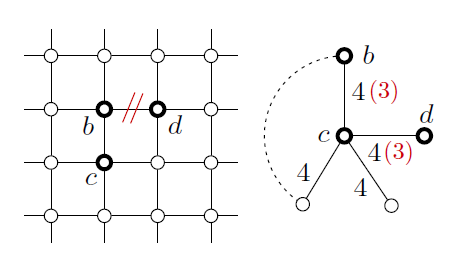
\includegraphics[width=\linewidth]{figures/Grid.png}
        \caption{Grid graph $G$ with star-shaped tree $T(G)$}.
        \label{Grid}
    \end{wrapfigure}

    it constitutes the worst-case with respect to an edge deletion or cost decrease. 
    
    Figure~\ref{Grid} shows an example based on a regular (unweighted) grid. In this example each vertex has degree 4, and we assum ethat the (global) edge connectivity is also 4. Then, the edge connectivity $\lambda_G(u,v)$ is also 4 for each vertex pair $\{u,v\}\subseteq V$, and $(\{u\},V\backslash\{u\})$ is a minimum \textit{u-v-}cut. Hence, any star with an arbitrary vertex $c$ as center and edges of cost 4 is a Gomory-Hu tree of G. Now assume the edge $\{b,d\}$ depicted in Figure~\ref{Grid} is deleted. For each vertex pair that contains at least $b$ or $d$, this decreases the connectivity to 3, however, the deletion has no effect on the connectivity of the remaining vertex pairs. Thus, decreasing the costs at the edges $\{c,b\}$ and $\{c,d\}$ in $T(G)$ would suffice to update the Gomory-Hu tree. Instead, Algorithm 4 checks each edge, apart from the two edges on $\pi (b,d)$, by computing a new minimum separating cut in $G^\ominus$. Consequently, it needs $n-3$ cut computations, which is the worst possible running time, as according to Lemma 4.3, maintaining the whole tree is possible if $\pi (b,d) = \{b,b\}$, or $\{b,d\}$ is a bridge.

    \clearpage
    \section{Limit on Fully Dynamic Algorithms}
    All known algorithms for computing Gomory-Hu Tree in a weighted graph make $\Omega(n)$ calls to an algorithm for the $s-t$ minimum cut problem. Thus, improved algorithms for constructing a Gomory-Hu Tree in a weighted graph have been corollaries of more efficient algorithms for the max. flow problem. \\
    
    Timothy G. Abbott and You Zhou proved that one of the two must happen [TY]:
    \begin{enumerate}
        \item {There are more efficient algorithms solving the Gomory-Hu problem than computing $n$ $s-t$ minimum cuts.}
        \item {There are no algorithms for dynamically maintaining the $s-t$ minimum cut in a weighted graph that are more efficient than the obvious algorithm of recomputing the cut from scratch on each query.}
    \end{enumerate}
    This is achieved using an explicit hardness relation showing that the problem of dynamically maintaining the s-t minimum cut is at least as hard as the problem of computing the  Gomory-Hu tree. This leaves open the possibility of efficient algorithms for dynamically maintaining the all-pairs $s-t$ minimum cut of a weighted graph.
    Throughout, it is assumed that all graphs are weighted graphs and all weights are non-negative. On a graph with $n$ vertices and $m$ edges, for simplicity, assume that $n = \mathcal{O}(m)$, as is the case of a connected graph.\\
    \indent
    Given a fully dynamic algorithm $A$ for the $s-t$ minimum cut problem on undirected graphs, with amortized query time $query_A(m, n)$, amortized update time $update_A(m, n)$, and initialization time $init_A(m, n)$, we give an efficient algorithm for constructing the Gomory-Hu tree on an undirected graph $G$. We assume all these time functions are monotonic and that they are bounded by a polynomial in the two inputs.
    Our data structure should support updates of adding or deleting an edge, along with adding or deleting a vertex other than $s$ and $t$ which has no edges attached to it. We will define the $s-t$ minimum cut query so that it returns the set defining one side of the cut, rather than simply the value of the cut or the edges cut.

    \vspace{5mm}
    \noindent{\large \bf Theorem 4.1:} \textit{If A is a fully dynamic algorithm for the $s-t$ mincut problem on an undirected graph, then with O(n · $query_A(m, n)+n$ · $update_A(m, n)+init_A(m, n)+n^2$) time, one can compute the Gomory-Hu tree for an undirected graph G with n vertices and m edges.}
    
    \vspace{5mm}
    \noindent{\large \bf Corollary 4.4:} \textit{If A is a fully dynamic algorithm for the s-t mincut problem, then with O(n · $query_A(m, n)+n$ · $update_A(m, n)+init_A(m, n)+n^2)$ time, one can compute the all-pairs minimum cut of an undirected graph G with n vertices and m edges.}

    \vspace{3mm}
    \noindent This shows in a strong sense, it is as hard to efficiently maintain the dynamic $s-t$ minimum cut as it is to compute the Gomory-Hu tree. 
    \clearpage
    \noindent The following theorem, equates the hardness of dynamically maintaining $s-t$ minimum cuts to the hardness of computing them in the static case, if current techniques for constructing Gomory-Hu trees from $s-t$ minimum cuts are optimal.

    \vspace{5mm}
    \noindent{\large \bf Theorem 4.2:} \textit{For any fully dynamic algorithm A maintaining the s-t minimum cut, one of the following must hold:
    \begin{enumerate}
        \item {The initialization time for A must be $\omega$(n · T(m, n)), where $T(m, n) = query_A(m, n) + update_A(m, n)$ is the larger of the update time for A and the query time for A.}
        \item {There are algorithms for computing the Gomory-Hu tree that are more efficient than O(n) s-t minimum cuts.}
        \item {A is no more efficient than computing the s-t minimum cut from scratch on each query.}
    \end{enumerate}
    }

    Since most efficient data structures do not require more than $n$ updates worth of time to initialize, Case 1 is a minor technical condition. Aside from this condition, this theorem implies that any dynamic algorithm for the $s-t$ minimum cut problem more efficient than recomputing from scratch on each query gives rise to a new, more efficient kind of algorithm for the Gomory-Hu tree problem. \\
    
    \noindent After removing the technical condition on initialization time for sparse graphs we have:
    
    \vspace{3mm}
    \noindent{\large \bf Corollary 4.5:} \textit{ For any fully dynamic algorithm A maintaining the s-t minimum cut on sparse graphs (where $m = \Theta(n)$), one of the following must hold:
    \begin{enumerate}
        \item {There are algorithms for computing the Gomory-Hu tree on sparse graphs that are more}
        \item {On sparse graphs, A is no more efficient than computing the s-t minimum cut from scratch on each query.}
    \end{enumerate}
    }

    \noindent Arikati et al. showed that one can efficiently compute the all-pairs minimum cut in sparse graphs when a certain topological property is small [Ari95], but in general there are no known algorithms for computing the Gomory-Hu tree in sparse graphs more efficiently than $n$ times the best algorithms for max flow in sparse graphs. \\
    We can similarly remove the technical condition on initialization times if we require the data structure to support bulk updates, in which a single operation supports adding or deleting a vertex along with all incident edges.

    \vspace{4mm}
    \noindent{\large \bf Corollary 4.6:} \textit{ For any fully dynamic algorithm A maintaining the s-t minimum cut and supporting bulk updates, one of the following must hold:
    \begin{enumerate}
        \item {There are algorithms for computing the Gomory-Hu tree that are more efficient than computing O(n) s-t minimum cuts.}
        \item {A is no more efficient than computing the s-t minimum cut from scratch on each query.}
    \end{enumerate}
    }

    % Developing efficient algorithms for dynamically maintaining the Gomory-Hu tree (or showing that they cannot exist) would be a good direction for future investigation.
    \chapter{Applications of Gomory-Hu Tree}
    After going through multiple research papers I observed that almost all, if not all applications of Static and Dynamic Gomory-Hu trees are on various Clustering Algorithms and Connectivity.

    \vspace{5mm}
    \noindent \textbf{Graph Clustering} problems aims at decomposing a given graph along sparse cuts into somewhat dense subgraphs called \textit{clusters}. It focuses on \textit{intra-cluster density} and \textit{inter-cluster sparsity}. Further clustering problems are used to get good heuristics in NP-hard problems that rely in finding good clusters.

    \begin{figure}[!htb]
        \centering
        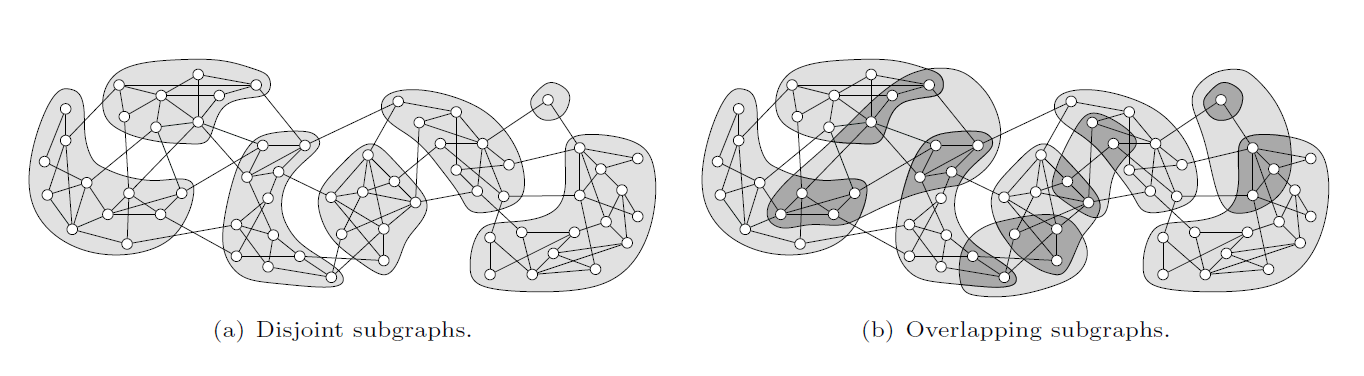
\includegraphics[width=1\linewidth]{figures/cluster.png}
        \caption{Decomposition of a graph into subgraphs}
        \label{cluster}
    \end{figure}
    \vspace{3mm}

    \noindent Some of the popular quality measure to measure clustering in a graph are - 
    
    \vspace{5mm}
    \noindent{\bf 1. Modularity} of clustering in an undirected unweighted graph is based on the total edge cost in $G$ that is covered by clusters with values ranging from -0.5 to 1, with 1 being the best value. Modularity $\mathcal{M}$ of a clustering $\Omega$ is defined as - 
    $$\mathcal{M}(\Omega) = \sum_{C\in \Omega}c(E_C)/c(E) - \sum_{C\in \Omega}(\sum_{v\in C} deg(v))^2/4c(E)$$ 

    \vspace{5mm}
    \noindent{\bf 2. Expansion} is a quality measure of cuts in weighted graphs. Higher the expansion the better. Expansion $\psi(U,C\backslash U)$ of a clustering $(U,C\backslash U)$ is defined as - 
    $$\psi(U,C\backslash U) = \frac{c(U,C\backslash U)}{min(|U|,|C\backslash U|)}$$ 

    \vspace{5mm}
    \noindent{\bf 3. Conductance} is a quality measure of cuts in weighted graphs. Lower the conductance the better. Condutance $\phi(U,C\backslash U)$ of a clustering $(U,C\backslash U)$ is defined as - 
    $$\phi(U,C\backslash U) = \frac{c(U,C\backslash U)}{min(deg(U),deg(C\backslash U)}$$ 

    \noindent Among the Cut-based Clustering techniques commonly used are - 
    
    \vspace{2mm}
    \noindent{\bf 1. Static Hierarchies of Cut Clustering} - Aim is to compute and organize all relevant minimum cuts of a graph into a nested hierarchical structure to form a hierarchy of clusters, so that the global cut structure of the graph can be further examined/analyzed. One algorithm for this was presented by Flake et al. that exploits the propoerties of minimum separating cut together with an input parameter $\alpha$ to find hierarchial clustering $C$.

    \vspace{5mm}
    \noindent{\bf 2. Maximum Source-Community Clustering} - identifies \textit{communities} in a graph by repeatedly finding min-Cuts that best separate a chosen vertex from the rest of the graph. It can be used for Community Detection, Hierarchial Clustering Tree, etc.

    \vspace{5mm}
    \noindent{\bf 3. Unrestricted Cut-Clustering Algorithm} Similar to previous one this also aims at finding communities in a graph but without any restrictions on the end vertices $s-t$.

    \vspace{5mm}
    \noindent{\bf 4. Fully Dynamic Hierarchies of Unrestricted Cut-Clustering Algorithm} Instead of a Static unrestricted Cut-Clustering, this one accommodates for mobility in the clusters do dynamically update and detect or erase newer clusters. Similar to Dynamic Gomory-Hu trees this one also supports concrete changes on a concrete edge and finding changes at each step.

    \vspace{5mm}
    Some of the major/significant Applications of Gomory-Hu Tree as given in various research papers are:
    \begin{enumerate}
        \item {
            \textbf{Image Segmentation [WL93]:} Given an input image our goal is to partition the image into various parts, such that each part has some meaningful interpretation. While there are many do Image Segmentation including usage of Convolutional Netural Networks, here we are going to Segment the image by converting it into a graph and partition based on Cut-values between nodes. \\ 
            More about this is discussed in the next chapter.
        }

        \item {
            \textbf{Identifying protein complexes in Protein-Protein Interaction(PPI) [JM20]:} Y2H (Yeast two-hybrind) PPI networks comprise proteins (nodes) and interactions of the type Y2H (edges). In the view of graph theory, a PPI network is an undirected and unweighted network. The intuition being - A protein complex should have strong internal connectivity and relatively weak external connectivity. \\
            Additionally, with the use of Sensitivity and Parametric analysis of Dynamic Gomory-Hu Trees one can efficiently filter out False Postives and Negatives. 
        }

        \item{
            \textbf{Optimal Service Component Distribution across Multiple Clouds [DA18]:} Service Request in a Multi-Cloud Model can be expressed as a complex topology with nodes and links constraints. The goal is to decompose the request into sub-request and try to minimize the number of partitions that can be mapped to at least one cloud provider meeting the user requirements. This decomposition step is done using Gomory-Hu Tree to cluster/parition into multiple clouds.
        }

        \item{
            \textbf{Finding All k-Edge-Connected Components [Tia15]:} Given a graph $G = (V, E)$, the problem is to partition the vertex set $V$ into ${V_1,V_2,. . ., V_h}$, where each $V_i$ is maximized, such that for any two vertices $x$ and $y$ in $V_i$, there are $k$ edge-disjoint paths connecting them.
        }

        \item{
            \textbf{Collaborative Uncapacitated Arc Routing Problem:} The goal is to maximize profit in a network with multiple carriers and each of them Collaboratively/Collectively work to optimize a given function (such as travel cost). Assuming that the nodes have no binding capacity constraints.
        }

        \item{
            \textbf{Graph b-coloring for Data Clustering [HH08]:} \textit{b-colouring} is a special case of \textit{proper b-colouring} where there exists a special vertex \textit{u (dominating vertex/b-vertex)} which is adjacent to at least one other vertex in every other colour class. This is used in Clustering since the \textit{b-vertex} can be used as a boundary object between two different classes and helps to distinguish clusters clearly.
        }

        \item{
            \textbf{Joint Interference and User Association Optimization in Cellular Wireless Networks [Cr13]:} In wireless networks users must connect to base stations. In modern network the best stations it not necessarily the nearest one. Here, we attempt to decompose the problem into smaller subproblems and then use min-cut to find bottlenecks and boundaries in the network.
        }
    \end{enumerate}
    \chapter{Image Segmentation}
    \textbf{Image segmentation} is a computer vision technique that partitions a digital image into distinct regions or pixel groups, assigning labels to every pixel to simplify image analysis and understand specific objects, boundaries, or features. It separates foreground objects from the background, enabling precise identification and localization of items. \\
    While there are many ways to do Image Segmentation such as Deep Learning, Neural Networks, Convolutional Neural networks and k-means clustering. Here we are going to use Cut-based Hierarchical clustering to segment images. 

    \section{Cut-based Clustering}
        The data to be clustered is represented by an undirected adjacency graph $G$ with arc capacities assigned to reflect the similarity between the linked vertices. Clustering is achieved by removing arcs of $G$ to form mutually exclusive subgraphs such that the largest inter-subgraph maximum flow is minimized. The segmentation is achieved by effectively searching for closed contours containing isolated strong edges, while rejecting contours containing isolated strong edges. This method is able to accurately guarantee the formation of closed edge contours.
        
        For the case of an unconstrained optimal $K-$subgraph partition of $G$, the arcs selected for removal are those in a set of $K-1$ minimum cuts with the smallest $K-1$ values among all possible minimum cuts separating all pairs of vertices. The resultant clustering achieved by this method is a globally optimal solution. It minimizes the largest inter-subgraph maximum flow among all possible $K-$partitions of $G$, hence minimizing the similarity between the subgraphs (clusters). The difficulty in reaching a globally optimal solution for a particular partitional clustering technique arises from the requirement that a huge number of $K-$ partitions must be considered.

        The following Clustering Strategy can be efficiently implemented to handle graphs of size ~$2000$ vertices. In addition, this clustering technique apart from optimal $K-$subgraph partition also produces a nested sequence of partitions which are optimal for cluster numbers ranging from $2$ to $K$. \\
        The following are the steps in the clustering method:
        \begin{enumerate}
            \item {
                Construct an adjacency graph $G$ which can produce meaningful clusters.
            }
            \item {
                Construct the Gomory-Hu (equivalent min-Cut) Tree $T^*$ of $G$. 
            }
            \item {
                The optimal $K-$partition of $G$ can be equivalently obtained by simply disconnecting the $K-1$ arcs in $T^*$ with the $K-1$ smallest arc capacities.
            }
            \item {
                Each partition of nodes obtained after separating the $K-1$ minimum arcs is a resultant cluster.
            }
        \end{enumerate}
        
        \noindent However, this quickly becomes infeasible for graphs of larger size ($\geq 10^4 $ nodes) due to polynomial complexity of the algorithm.

        To overcome this problem Zhenyu Wu and Lichard Leahy present a faster hierarchical algorithm [WL93]. \\
        We are going to discuss about the algorithm in the next Section.

    \section{Hierarchical Clustering Algorithm}
        This algorithm requires construction and partition of a partially equivalent tree $T^*_c$ of greatly reduced size. This still results in an optimal solution equivalent to that obtained by partitioning the complete equivalent tree of $G$. The algorithm is based on the observation that most of the minimum cuts found in $G$ are never used since their associated cut-values are sufficiently large that the arcs in those cuts will not be removed to form subgraphs.

        \subsection{Formulation and Clustering Rationale}
            Here, it is assumed that the data set can be adequately represented by an adjacency graph $G$, where each vertex corresponds to a data point and an edge indicates a neighborhood relationship between the two linked components, and a similarity measure between these two is assigned to the arc as its flow capacity. \\
            In case of Image Segmentation one could construct such a graph in which each vertex represents a pixel in the image and edges are placed between pairs of neigbouring pixels.

            Let $G = (V,E)$ be an adjacency graph, formed from the data set with vertex $V = \{v_i,v_2,...,v_n\}$ and edge set $E = \{e_{ij}\}$ with $e_{ij}$ denoting the edge between vertices $v_i$ and $v_j$ with capacity $c_{ij}$. Here, $c_{ij}$ is a similarity measure between $v_i$ and $v_j$, i.e. the larger the edge capacity $c_{ij}$, the more similar are the vertices.

            \vspace{5mm}
            \noindent{\large \bf Theorem 6.1:} \textit{Let $G^* = (V,E^*)$ be a hypothetical complete graph with
            edge capacity $e^*_{ij} \in A^*$ equal to the maximum flow $F_{ij}$ betwen the corresponding vertices $v_i$ and $v_j$ of the original graph $G$. Then $T^*$ is flow-equivalent to the original graph $G$. Furthermore, the flow-equivalent tree $T^*$ is constructed using the Gomory-Hu algorithm is also cut-equivalent to $G$.
            }

            \vspace{5mm}
            \noindent{\large \bf Corollary 6.1 (to Theorem 6.1):} \textit{
                The $K-$partition of an undirected graph $G$, obtained by removing the $K-1$ edges with the smallest capacity in the equivalent tree $T^*$ of $G$, minimizes the largest inter-subgraph maximum flow among all possible $K-$partitions of $G$.
            }

            \vspace{5mm}
            \noindent{\large \bf Corollary 6.2 (to Theorem 6.1):} \textit{
                The $K-$partition of an undirected graph $G$, obtained by removing the $K-1$ edges with the smallest capacity in the equivalent tree $T^*$ of $G$, is unique if all K-1 edges in $T^*$ marked for removal have capacity strictly less than the remaining unmarked edges.
            }

            \vspace{3mm}
            \noindent As the number of subgraphs increases, so does the number of corresponding regions in the segmented image. Since the goal of clustering is to produce a small number of regions from the image, a stopping condition should be used to prevent for formation of too many regions. This could be achieved either interactively by terminating the edge cutting procedure when sufficient regions have been formed, or by using a threshold so that arcs with maximum flow above a given threshold are not cut. The problem os systematically choosing a suitable threshold is clearly important.

            The capacities may be any nonnegative symmetric function. In this case the following capacity function is used: \\
            \begin{center}
                $c_{ij} = k_{ij} \ \cdot \ e^{-(\frac{\mu_i - \mu_j}{\sigma})^2}$
            \end{center} 

            \noindent $k_{ij}$ denotes the number of neighboring pixels between vertices $v_i$ and $v_j$, \\
            $\mu_i$ and $\mu_j$ are the means of patches $i$ and $j$.

            \vspace{5mm}
            \noindent{\large \bf Theorem 6.2:} \textit {
                Let $G_o$ be a subgraph of an undirected graph $G$, and $F_{o,min}$ be the minimum value of the maximum flows between all pairs of vertices in $G_o$. Lets and t be an arbitrary pair of vertices in G such that the value of the maximum flow between s and t, $F_{st}$, is smaller than $F_{o,min}$. Then $F_{st}$ can be equivalently computed from the graph, $G_c$, which is obtained by condensing all vertices of $G_o$ into a single vertex.
            }

            \vspace{5mm}
            \noindent{\large \bf Corollary 6.3 (to Theorem 6.2):} \textit {
                Let $G_o$ be a subgraph of an undirected graph G. Let $F_{o,min}$ be the minimum value of the maximum flows between all pairs of vertices in $G_o$ computed using an arbitrary subgraph, $G_o$, which contains $G_o$, and let s and t be an arbitrary pair of vertices in G. If the value, $F_{st}$, of the maximum flow between s and t, computed using G, is smaller than $F_{o,min}$, then $F_{st}$ can be equivalently computed from the condensed graph $G_c$ with all vertices in $G_o$ condensed into a single vertex.
            }

            \vspace{2mm}
            \noindent The implication of Corollary 6.3 is significant since the condition under which a subgraph $G_o$, may be condensed can be checked using only a local subgraph which contains $G_o$.

            \vspace{5mm}
            \noindent{\large \bf Lemma 6.1:} \textit {
                Let $G_o$ be a subgraph of an undirected graph G, and $F^{'}_{st}$ be the value of the maximum flow between a pair of vertices, s and t, in $G_o$ computed using $G_o$. Let $F_{st}$ be the maximum flow between s and t computed using G. Then  $F{'}_{st} \leq F_{st}$.
            }

            \vspace{5mm}
            \noindent{\large \bf Theorem 6.3:} \textit {
                Let $G_o$ be a subgraph of an undirected graph G, and $F^{'}_{o,min}$ be the minimum value of the maximum flows between all pairs of vertices in $G_o$ computed in a subgraph $G^{'}_o$ which contains $G_o$. Let $G_c$ be the graph formed from G with all vertices in $G_o$ condensed into a single vertex and let $T^*_c$ is a partially cut and flow equivalent tree of G, at threshold $F^{'}_{o,min}$, in the sense that the maximum flow, $F_{st}$, and the corresponding minimum cut can be computed from $T^*_c$ for all pairs of vertices s and t in G such that $F_{st} \leq F^{'}_{o,min}$. Furthermore for all vertex pairs, s and t, in G with flow $F_{st} \geq F^{'}_{o,min}$, the maximum flow value computed in $T_c$ is also greater than or equal to $F^{'}_{o,min}$. 
            }

            \vspace{2mm}
            \noindent An \textbf{interior vertex} of a subgraph $G^{'}_o$ of $G$ is a vertex such that all of its neighbouring vertices also belong to $G^{'}_o$. A non-interior vertex is called a \textbf{boundary vertex}.

            \vspace{5mm}
            \noindent{\large \bf Theorem 6.4:} \textit {
                Let $T^{'*}_o$ be an equivalent tree of $G^{'}_o$, a subgraph of an undirected graph G, and $T^*_o$ be a branch of $T^{'*}_o$ consisting exclusively of interior vertices of $G^{'}_o$. Let $G_c$ be the graph formed from G, with all vertices in $T^*_o$ condensed into a single vertex $v^*_o$. The equivalent tree $T^*$ of G can be constructed as follows: \\
                Construct an equivalent tree $T^*_c$ for the condensed graph $G_c$, and then replace the vertex $v^*_o$ by $T^*_o$ connected at its root vertex.
            }

            \vspace{2mm}
            \noindent Here, the \textbf{root vertex} of the branch $T^*_o$ refers to the only vertex in $T^*_o$ which neighbors a boundary vertex in $T^{'*}_o$.


        \subsection{Implementation}

            \vspace{3mm}
            \noindent \textbf{Step 1)} Form the adjacency graph $G$, and then arbitrarily partition $G$ into a number of small subgraphs {$G^{'}_{0,m}$}, usually of similar size. Let $i=0$.
            
            \vspace{3mm}
            \noindent \textbf{Step 2)} For each subgraph $G^{'}_{i,m}$ find an equivalent tree $T^{'}_{i,m}$ using the Gomory-Hu algorithm.
            
            \vspace{3mm}
            \noindent \textbf{Step 3(i)} Permanently condense all the subtrees in $T^{'}_{i,m}$ which are linked by edges with capacities $\geq F_T$.
            
            \noindent \textbf{Step 3(ii)} Temporarily condense all the maximal interior branches of this resulting tree to form a condensed subgraph $G^{'}_{i,m,c}$.
            
            \vspace{3mm}
            \noindent \textbf{Step 4)}  If there is only one subgraph in {$G^{'}_{i,m,c}$}, then denote the resulting equivalent tree as $T^{'*}_c$ and go to Step 6. \\
            Otherwise continue to Step 5.
            
            \vspace{3mm}
            \noindent \textbf{Step 5)} Group {$G^{'}_{i,m,c}$} into subsets, each containing a number of neigbouring subgraphs of {$G^{'}_{i,m,c}$}. By connecting the subgraphs in each subset using the inter-subgraph edges, we form a new subgraph set ${G^{'}_{i+1,m}}$. Let $i = i+1$, and go to Step 2.
            
            \vspace{3mm}
            \noindent \textbf{Step 6)} Expand back all the temporarily condensed vertices in $T^{'*}_c$ to construct the partially equivalent tree $T^*_c$ of the original graph $G$.
            
            \vspace{3mm}
            \noindent \textbf{Step 7)} Remove successively edges in $T^*_c$ in order of increasing edge capacity until a given stopping condition is met. A clustering constraint may also be attached in this last step.

            \vspace{5mm}
            \noindent Since constructing an equivalent tree for graphs with few vertices is very fast, it is usually more efficient to start the algorithm with a large number of very small subgraphs. The only restriction in selecting the threshold $F_T$ is that no minimum cut with value larger than $F_T$ may be used for partitioning the graph $G$. Ideally the threshold $F_T$ should be chosen as the value of the largest minimum cut which will be made in partitioning $G$ so that the clustering is most efficient.


        \section{Results and Improvements}
        In this section I am going to discuss and show the results of the final Segmented Image on different categories of Image as generated by the above mentioned Algorithm. Furthermore, I am going to provide some of my own improvements to the above algorithm (keeping the core algorithm same) to achieve a better Runtime and also to improve the final Clustered images, to produce better results. \\
        The methods discussed above (in the paper [WL93]) were for Black-and-White images having a single parameter (intensity) describing each image. \\
        Here, I extended this to support RGB images having 3 parameters per pixel by using edge capacity function (between 2 pixels sharing an edge) as:-
        \begin{center}
            $c_{ij} = e^{-(\frac{\sum_{k=1}^{C}(\mu^k_i - \mu^k_j)^2}{C \ \cdot \ \sigma^2})}$
        \end{center}
        where C is the number of Channels (parameters per pixel).

        \vspace{7mm}
        \noindent \textbf{1. Synthetic Images (generated using MS Paint)}
        \begin{figure}[H]
            \centering
            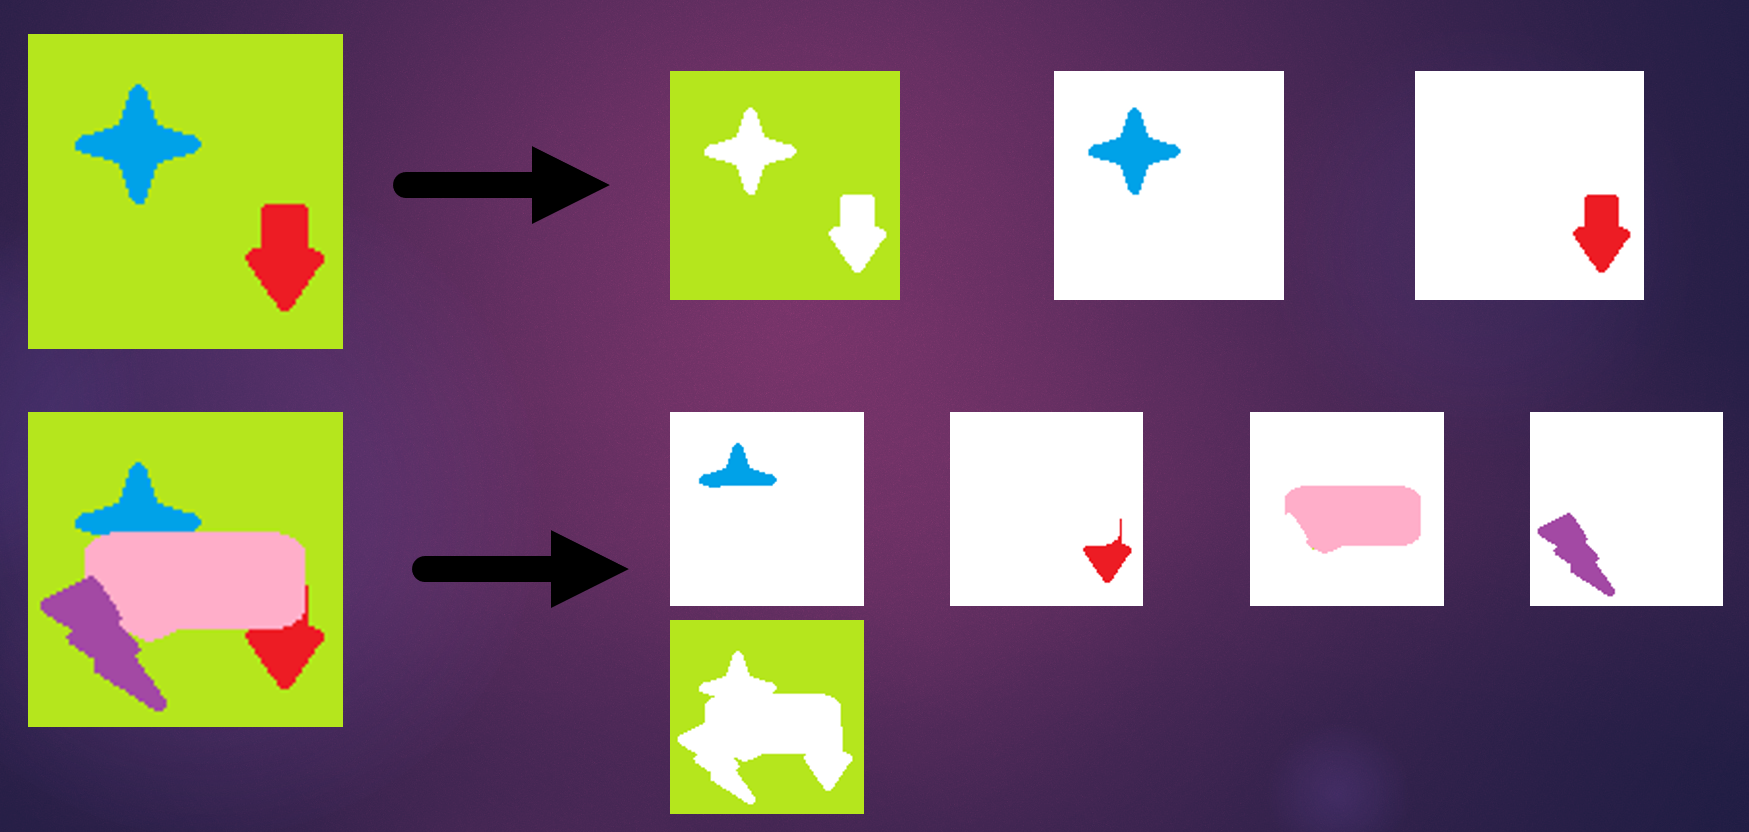
\includegraphics[width=1\linewidth]{figures/Synthetic_image.png}
            \caption{Synthetic Image}
            \label{fig:placeholder}
        \end{figure}

        \noindent We observe that \textbf{Synthetic Images} are separated very well by the Algorithm without any further modifications or improvements to it. All the elements in the image are properly segmented including the background.

        \clearpage
        \noindent \textbf{2. Real Images (high colour gradient)}
        \begin{figure}[H]
            \centering
            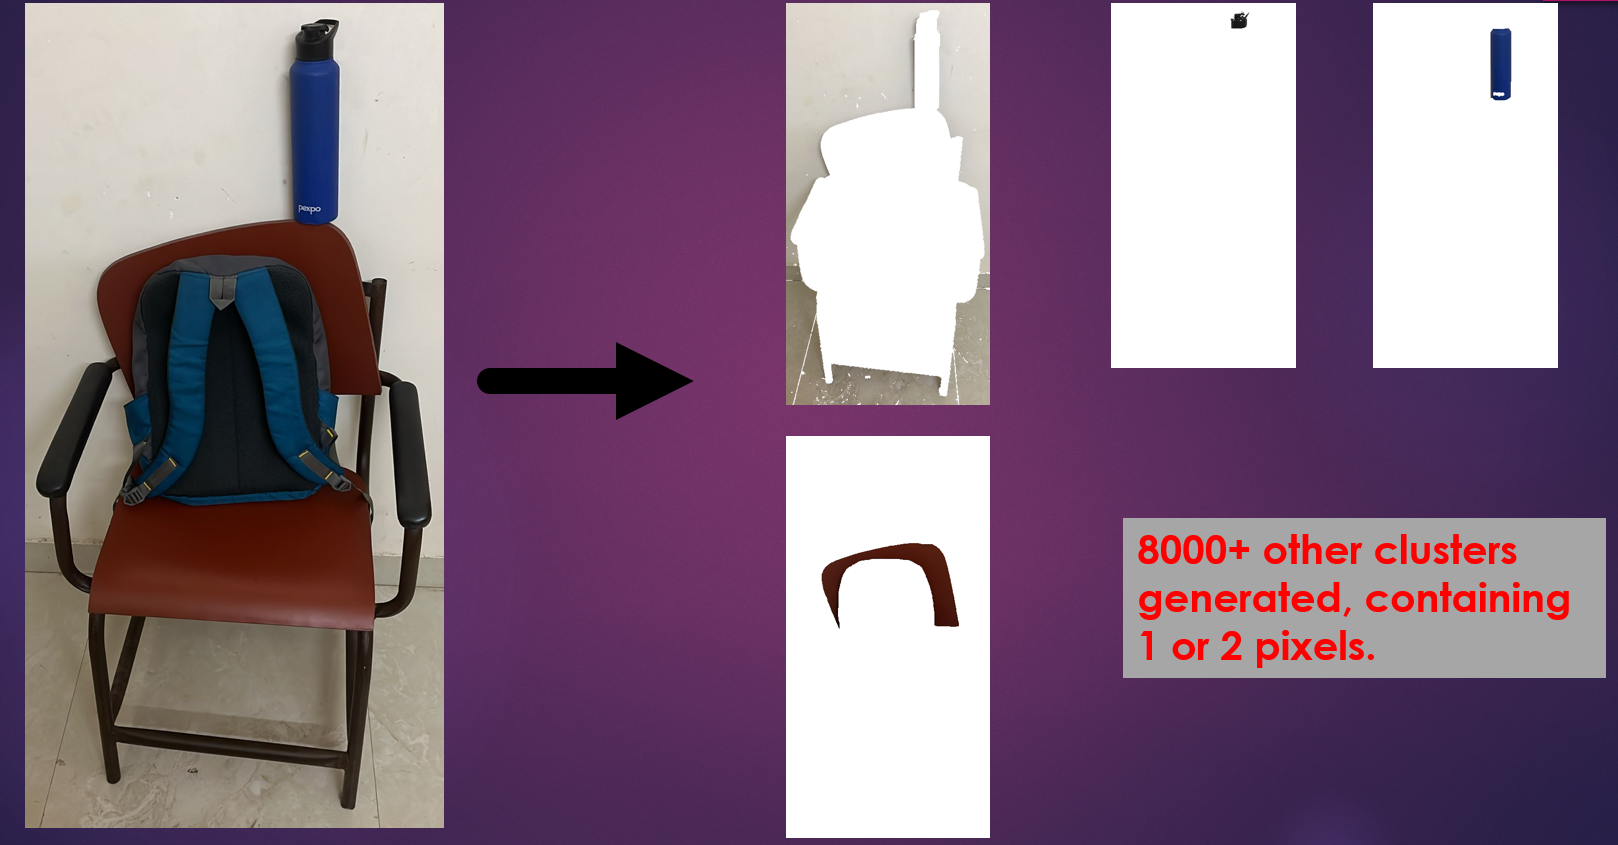
\includegraphics[width=1\linewidth]{figures/Real_Image_1.png}
            \caption{Real Images (having high colour gradient)}
            \label{fig:placeholder}
        \end{figure}

        \noindent In case of a \textbf{Real Image} even though the background separation and other components seem to be properly separated, there are more than 8000 clusters generated from this Image, which is not the Segmentation that we want to achieve.

        \vspace{3mm}
        \noindent \textbf{Reason:} The primary reason behind this is the Algorithm separates first the easily \indent \indent \indent \indent \indent separable clusters. \\
        Consider the the case where there is a very small black speck present in a white background. Now, we don't want to separate that part of image since that is just some error/variance in the image which we would like to ignore. However, since black and white generate the highest contrast and as a result the edge capacities between then will be very low and also a very low min-Cut value. This results in separation of that speck and is treated as a separate cluster.

        \vspace{5mm}
        \noindent \textbf{Improvement-1: } Setting lower limit on the the number of nodes/pixels that should be \indent \indent \indent \indent \indent \indent \indent \indent \indent present in a cluster. \\
        This is ensured by a merge step after the initial partition, where for each cluster having $\leq MIN\_SIZE$ nodes/pixels in a cluster is merged to another cluster which bears the highest similarity (max. min-Cut) to the current cluster.

        \begin{figure}[H]
            \centering
            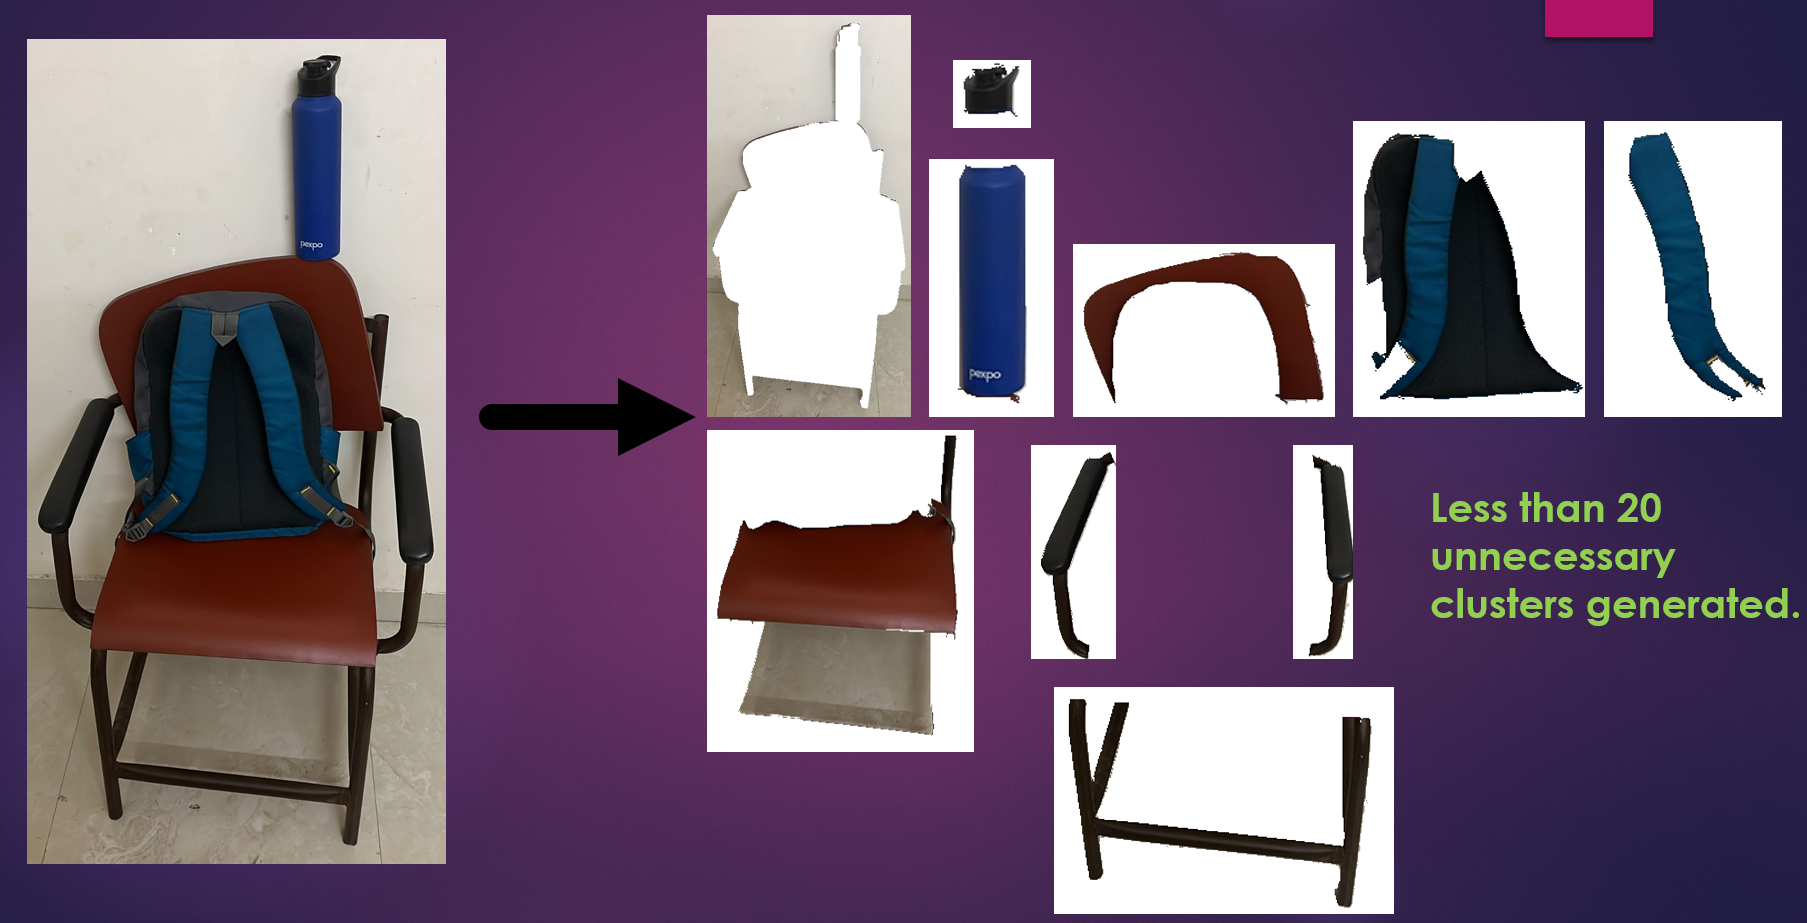
\includegraphics[width=1\linewidth]{figures/Real_Image_after_Improvement_1.png}
            \caption{Real Image (after Improvement-1)}
            \label{fig:placeholder}
        \end{figure}

        \vspace{2mm}
        \noindent Here we observe that after implementing Improvement-1 for minimum Cluster size all the major elements for the Image are now properly separated. Furthermore, there are only less than 20 other clusters apart from the main ones (containing physical elements) which appear to be useless compared to the 8000+ clusters from previous case.

        \vspace{7mm}
        \noindent \textbf{3. Natural Images}
        \begin{figure}[H]
            \centering
            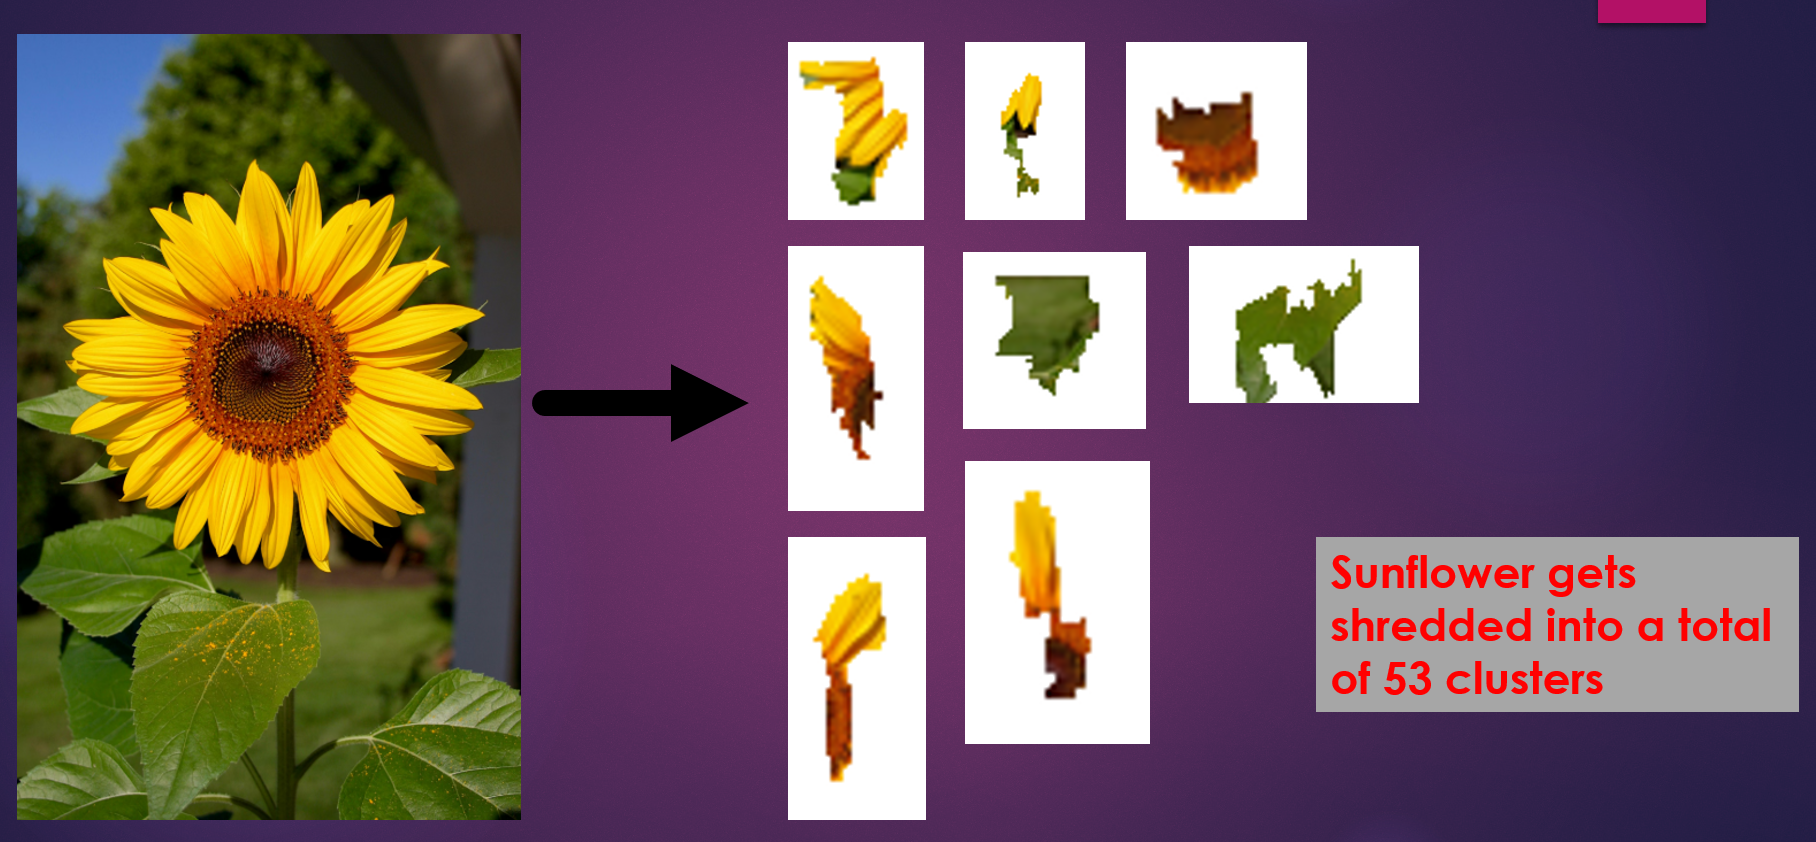
\includegraphics[width=1\linewidth]{figures/Natural_Image_1.png}
            \caption{Natural Image - 1}
            \label{fig:placeholder}
        \end{figure}

        \vspace{2mm}
        \noindent In case of this Natural Image containing a sunflower with some background in it, we see that the Sunflower gets shredded into multiple different parts and the parts(clusters) of it also don't have any meaningful physical interpretation.

        \vspace{3mm}
        \noindent \textbf{Reason:} Most likely the reason behind this is that the pixels don't have enough contextual information to perform the clustering. Taking only adjacent pixels as edges in case of Natural Images is not enough context to perform the clustering.

        \vspace{5mm}
        \noindent \textbf{Improvement-2: } Instead of only taking Orthogonal adjacent pixels as edges, increase the Neighborhood size to 3 or 5 pixels surrounding it and also optionally adding diagonal edges to add more surrounding context for the current pixel. \\ 
        Even though this Improvement results in better overall clustering it also affects the execution time for Clustering since increasing neighbourhood also means increasing the number of edges in the graph.

        \begin{figure}[H]
            \centering
            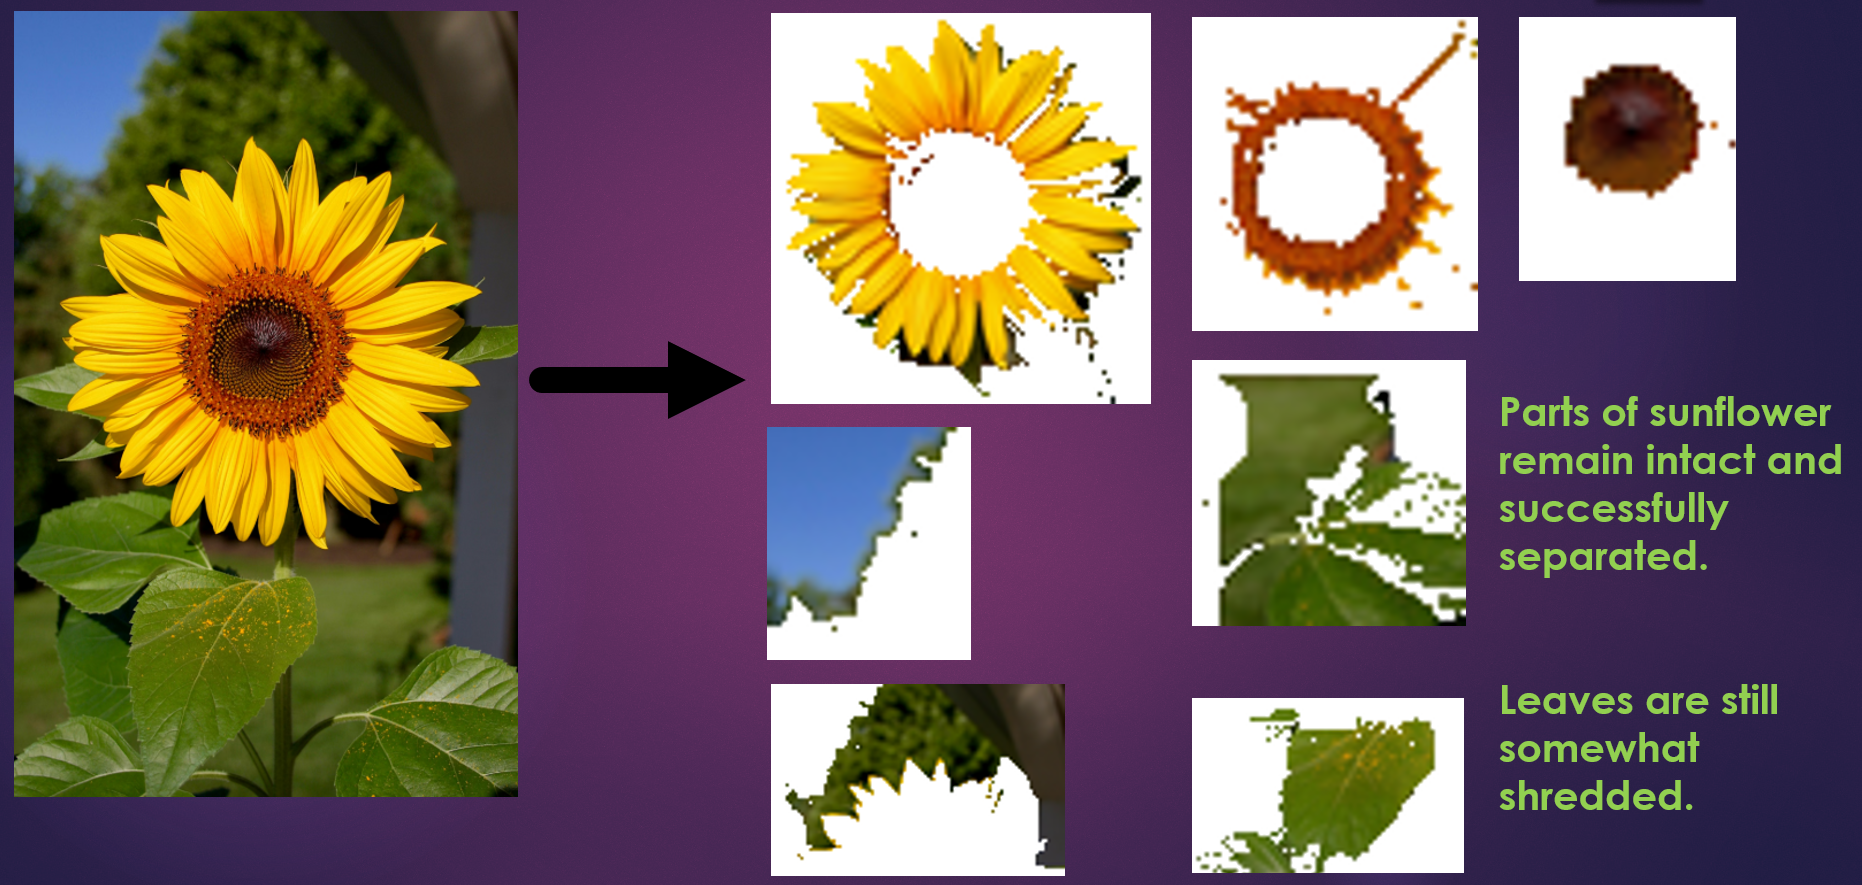
\includegraphics[width=1\linewidth]{figures/Natural_Image_1_after_Improvement2.png}
            \caption{Natural Image - 1 (after Improvement-2)}
            \label{fig:placeholder}
        \end{figure}

        \vspace{2mm}
        \noindent After Implementing Improvement-2, now we see that Segmentation is much better. Sunflower instead of getting shredded into pieces is now divided into 3 parts (Outer part having Yellow petals, Middle Orange Ring and the Inner Brown Core part). The background sky and other parts are also somewhat separated. \\
        Leaves are better clustered although the leaves are still somewhat shredded. This is because of poor/low colour gradient i.e. Green Leaves in a Green Background.

        \clearpage
        \subsection{Execution Time Improvements}
            Till now we have discussed improvements for better resultant Clustering. \\
            Here, I am going to provide a few methods to optimize the overall Execution Time required to generate the final Clusters from the Initial Input Image.

            \begin{enumerate}
                \item {
                    \textbf{Parallelizing Local Subgraph Computation:} Observe that Step 2 (from SubSection 6.2.2 - Implementation) - computing Gomory-Hu Tree for each local subgraph is independent for each of the local subgraphs $G^{'}_{i,m}$. \\ 
                    Here, we can divide the computation of different $T^{'}_{i,m}$ into different threads i.e. for a given Hierarchy Level $i$ we can parallelize over the values of $m$.
                }
                \item{
                    \textbf{Mathematically finding Optimal Hierarchy Depth:} Instead of going for Higher levels of hierarchy and subgraph merging until the no. of subgraphs becomes 1 (Step 4 - first case), we can stop at an earlier Level if we observe that there are very few Node or Edge condensations in the graph. Unnecessarily going for higher levels of Hierarchy without significant Node/Edge condensations just leads extra computation time. This in-turn results in a worse overall computation time than the trivial Cut-based Clustering approach as discussed earlier. \\
                    Consider the analogy in the case of FFT (Fast-Fourier Transform) where we stop at a base case if the two vectors to be multiplied have sizes less than a certain value and compute that case using the Trivial Brute Force Multiplication Approach.                    
                }
                \item{
                    \textbf{Maintaining Bipartiteness after each Condensation Step:} Since the initial graph generated from the Image is a lattice graph and is therefore Bipartite, we can attempt to preserve this Bipartiteness property of the Graph throughout the Clustering process. This helps because when computing the Gomory-Hu Tree and we are doing $n-1$ flow computations. In case of Bipartite graphs Worst Case flow computation time = $O(E\sqrt{V})$. Also, since the graphs generated from images are sparse graphs i.e. $E = O(V)$, we have overall worst case Gomory-Hu Tree construction time:-    $O((V-1)\ \cdot \ E\sqrt{V}) = O(V \ \cdot \ V\sqrt{V}) = O(V^2\sqrt{V})$. \\
                    However, there are 2 issues with this:
                    \begin{itemize}
                        \item {
                            Since, we are trying to maintain bipartiteness at each Step, number of Edge Condensation will always be = 0. \\
                            Because, if two adjacent nodes sharing an edge are condensed into a single node then bipartiteness property will be broken. Also, since the Condensations are constrained, this also results in lower Node condesations. So overall, this method even though has better worst case time might lead to worse overall execution time due to lower Node/Edge Condensations.
                        }
                        \item {
                            Dinic's algorithm which is used for Flow computation here already has very low flow computation time on average. So, improvement in asymptotics might not be a very high improvement over Dinic's average case complexity. Even though it has a worst case time of $O(V^2E)$, for most cases it works below $O(V^2)$ overshadowing any significant improvement in computation times.
                        }
                    \end{itemize}
                }
            \end{enumerate}

        \subsection{Other Improvements}
            Apart from \textbf{Improvement-1} and \textbf{Improvement-2} presented previously, here I provide some other possible additional improvements which might lead to better Final Clustering.

            \begin{enumerate}
                \item {
                    \textbf{Optimally choosing Hyperparameters based on the input image rather than Hardcoding:} There are several Hyperparameters present in the Implementation such as - \textit{WINDOW\_SIZE, THRESHOLD, MIN\_CLUSTER\_SIZE, NEIGHBOURHOOD}. Instead of fixing those values as compile-time we can find an optimal configuration of these Hyperparameters based on the Input Image, since different Images have different requirements. \\
                    E.g- A higher Resolution image will most likely need a higher MIN\_CLUSTER\_SIZE compared to a lower one. \\
                    Choosing THRESHOLD based on the color gradients of the Image and then choosing the edge value at say the $10^{th}$ percentile.
                }
                \item {
                    \textbf{Processing input separately for R,G,B Channels and then combining them:} Instead of generating an edge capacity based on the difference between R,G,B intensities of 2 pixels and summing then up we can divide the image into 3 parts and then construct separate clusterings for the 3 parts. Finally, using some heuristic we can combine all those clusterings to generate a final clustering. \\
                    This is further enchanced by the fact that the core algorithm for this clustering was built for single Channel (greyscale) images. Dividing up the image effectively ensures each individual Channel is a greyscale (single parameter per pixel) image.
                }
                \item {
                    \textbf{Capacity function based on the type of Image:} We are using the same capacity function for all types of Images irrespective of their final goals. \\
                    Instead of that we can choose different capacity functions based on the type of Image (Greyscale, Synthetic, Real or other Natural Image) and the final aim of Clustering to potentially further improve the clusters.
                }
            \end{enumerate}


    \section{Advantages}
        Major advantages to the above mentioned Clustering technique primarily are:-
        \begin{enumerate}
            \item {
                \textbf{Unsupervised:} Unlike ML models, no previous training data or labelled dataset is needed for clustering the Images.
            }
            \item {
                Since, Learning is Unsupervised there is no training time required for previous computations. We can directly process Images without any previous inputs.   
            }
            \item {
                If the Image has large potions of similar coloured regions, there will be high Node/Edge condensations. In those cases, overall execution time will be very low due to extremely reduced size of final condensed graph.
            }
        \end{enumerate}

    \section{Drawbacks}
        Along with the above discussed Advantages, this Hierarchical Clustering method also has some serious (major) Drawbacks and Disadvantages some of which are tied intricately to the functioning of the core algorithm.

        \begin{enumerate}
            \item {
                \textbf{Poor results in case of Natural Images:} This method of clustering basically relies on high contrast between colours in neighbouring pixels for Segmentation/Clustering. Natural Images generally tend to have a low colour gradient. In those cases it becomes especially hard to segment out various parts of the Image.
                \begin{figure}[H]
                    \centering
                    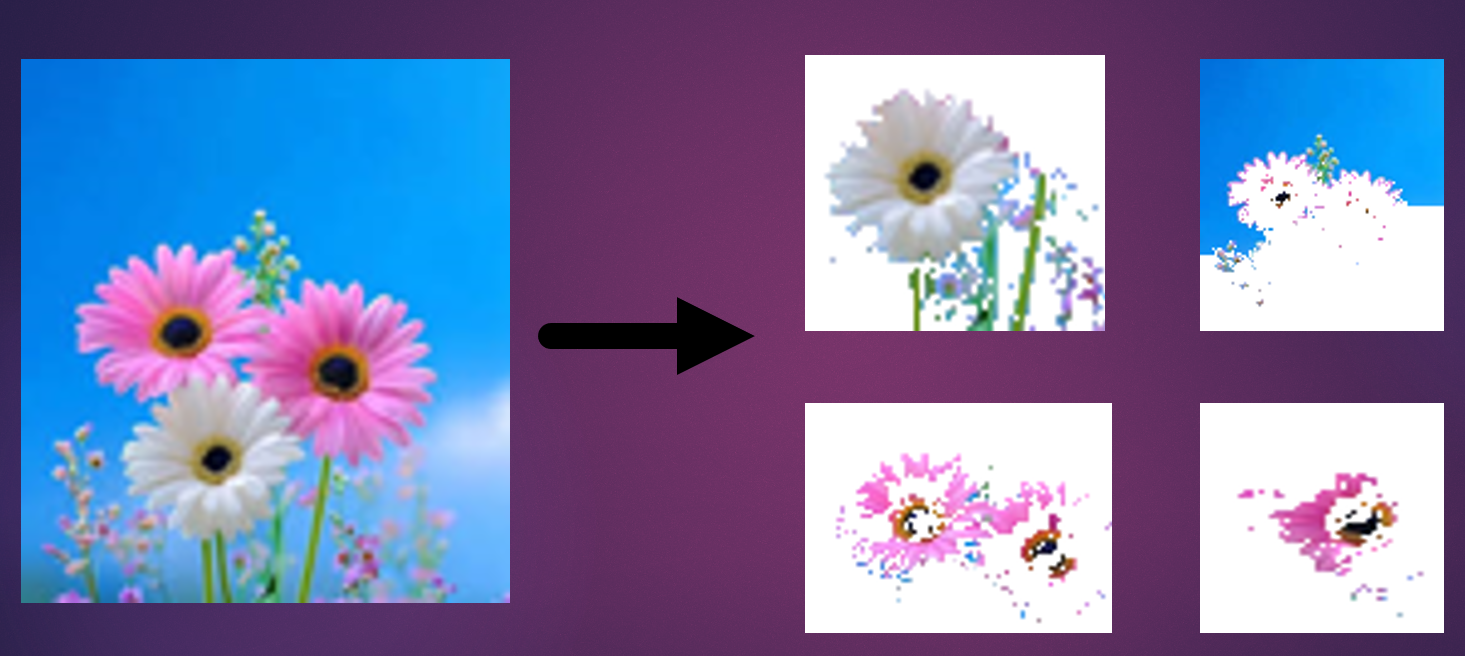
\includegraphics[width=1\linewidth]{figures/Natural_Image_2.png}
                    \caption{Natural Image - 2 (Somewhat unsuccessful Segmentation)}
                    \label{fig:placeholder}
                \end{figure}
                We can see that among the 3 flowers in the image only the White one having the highest contrast was properly Segmented along with the background Sky. It completely failed as segmenting the other 2 flowers with low Contrast.
            }
            \item {
                For higher resolution images such as 1k, 2k or 4k the number of nodes in the graph is very high (multi-millions) and as a result the execution time is also very high.
            }
            \item {
                \textbf{Lack of Context (Over-Segmentation):} A single object having different colours in different regions will be segmented into various parts (clusters), since the primary objective of this algorithm is to "Cluster on the basis of Colour". \\
                However, this might not be the expected result in most real-life scenarios as we generally want to keep the object as a whole and separate one object from another, rather than "One colour from Another". \\
                In that case we need more context signifying that the parts of a single object are related to one another and should be kept within a single cluster. This however, relates more to (and is solved by) ML-based Clustering, and is a fundamental drawback of Cut-based Image Segmentation algorithms.
            }
        \end{enumerate}
    \chapter{Future Work}
    The following are some of the possibilities of continuation to my current work in the area of Static and Dynamic Gomory-Hu Tree and their Applications, for the upcoming Semester/Year for MTP (M.Tech Project):-

    \vspace{5mm}
    \begin{enumerate}
        \item {
            Further exploring Cut-based Image Segmentation and trying to improve for better execution times and overall more accurate final Clusters.
        }
        \item{
            Extending Dynamic Gomory-Hu Tree to multiple edge-updates instead of single-update, given that the updates are Offline i.e. known to us beforehand.
        }
        \item {
            Exploring and Improving Dynamic Gomory-Hu Tree for specific special graph types. Instead of going into improving Dynamic Gomory-Hu Tree for general graphs as a whole, I can take some special graph type and then try to improve Dynamic Gomory-Hu Tree for that specific case.
        }
        \item {
            Theoretically determining beforehand, the number of newer flow computations required in case of decreasing edge weights in Dynamic Gomory-Hu Tree. \\
            The current Decreasing Edge Weight algorithm for Dynamic Gomory-Hu Tree as proposed by T. Hartmann and D. Wagner (2013) [HT13] only gives an upper bound as to how many newer flow computations the algorithm will perform, the exact value is known only after fully performing the updates. \\
            Instead of this, I can attempt to mathematically/theoretically determine the number of newer flow computations that will be done by this algorithm without actually doing the update.
        }
        \item {
            Finally, I can explore other Applications of Gomory-Hu Tree apart from Image Segmentation such as - Network Reliability and Sensitivity Analysis or Community Detection.
        }
    \end{enumerate}

    \nocite{*}
	\bibliographystyle{alpha}
	\bibliography{bibliography}
	
	
\end{document}